% !TeX spellcheck = Greek_Caps_English_US
\documentclass[article,a4paper,12.7pt]{memoir}


\usepackage{graphicx}
\usepackage{placeins}
%\usepackage{sidenotes}
%\usepackage[a4paper,left=24.8mm,top=27.4mm,headsep=2\baselineskip,textwidth=107mm,
%					marginparsep=8.2mm,marginparwidth=49.4mm,textheight=49\baselineskip,
%					headheight=\baselineskip]{geometry} % tufte-handout definitions
\usepackage[a4paper,
left=22mm,top=27.4mm,
headsep=2\baselineskip,
textwidth=107mm, %110mm
marginparsep=6.0mm, %4.0mm
marginparwidth=70mm, %70mm
textheight=52\baselineskip,
headheight=\baselineskip]{geometry} % tufte-handout definitions

%=======Fonts and Language [XelateX only]=====
\usepackage{fontspec}
\usepackage{float}
\usepackage{morefloats}
\usepackage{polyglossia}
\usepackage{svg}

\setmainlanguage{greek}
\setotherlanguage{english}
\setmainfont{Liberation Serif}
\newfontfamily\greekfont{Liberation Serif}
\newfontfamily\greekfontsf{Liberation Serif}
\newfontfamily\greekfonttt{Liberation Serif}

%====Physics and Maths Symbols=============
\usepackage{amsmath}
\usepackage{amssymb}
\usepackage{xparse}
%\usepackage[arrowdel]{physicsrev} %Physics Packge (Revised)
\usepackage[arrowdel]{physics}
\usepackage[version=3]{mhchem} %Chemistry Symbols
\usepackage{wasysym} %Astronomical Symbols

\usepackage{siunitx} %Units
\usepackage{cancel}
\usepackage{multirow}
%=====Graphics=============
\usepackage{graphicx}
%\usepackage{caption}
\usepackage{lipsum, calc, needspace}
%\usepackage{subcaption}
\usepackage{textcomp}
%\usepackage{tikz}
\usepackage{scrextend}
%============================
\newlength\widthw
\setlength{\widthw}{\textwidth+\marginparsep+\marginparwidth}


\newlength{\fullwidthlen}
\setlength{\fullwidthlen}{\marginparwidth}
\addtolength{\fullwidthlen}{\marginparsep}

\newenvironment{fullwidth}{%
	\begin{adjustwidth*}{\ifthispageodd{-5cm}{-0cm}}{\ifthispageodd{-0cm}{-5cm}}%
	}{%
	\end{adjustwidth*}%
}

%======Other==============
\usepackage{multirow}
\usepackage{booktabs}
\usepackage{latexsym,graphicx}
\usepackage{todonotes}
%\usepackage{xcolor}
%\usepackage[some]{background}
%\usepackage{wrapfig}
%\usepackage{sidecap}
%\usepackage{lscape}
%\usepackage{rotating}
%\usepackage{geometry}

%===Bibliography======================
\usepackage[backend=biber,style=authoryear,citestyle=authoryear]{biblatex}
%\addbibresource{My Library.bib}

%=========Unit Declaration==========
\DeclareSIUnit \cm {\centi\meter}
\newcommand{\sm}{$M_{\odot}$}

\title{Αριθμητικές προσομοιώσεις νεφών σε γαλαξίες}
\author{Παπαχρήστου Μιχάλης}

\numberwithin{equation}{subsection}
\setsecnumdepth{chapter}
\setcounter{secnumdepth}{3}
\counterwithout{section}{chapter}
\newcommand{\tabletodo}[3][]{\begin{minipage}{#2}\todo[inline,#1]{#3}\end{minipage}}



\begin{document}
\sisetup{retain-unity-mantissa = false,range-phrase=\texttt{ έως },range-units = single,separate-uncertainty = true}

	\maketitle
	Σε αυτή την εργασία θα προσπαθήσουμε να μελετήσουμε μέσω αριθμητικών εξομοιώσεων τη δυναμική ενός μοριακού νέφους (MC) μέσα στο διαγαλαξιακό μέσο (ISM). Για τις αριθμητικές εξομοιώσεις θα χρησιμοποιήσουμε τον κώδικα PLUTO (\cite{mignone_pluto:_2007})  ώστε να μελετήσουμε μια όσο το δυνατόν ρεαλιστικότερη απεικόνιση ενός σφαιρικού μοριακού νέφους χτίζοντας την, βήμα βήμα μέσω διαφορετικών φυσικών διεργασιών (Radiative Cooling. Magnetic Fields, Gravity, etc)
\section{Μοριακά Νέφη και διαγαλαξιακός χώρος}
Στον μεσοαστρικό χώρο υπάρχει μια τεράστια ποσότητα ύλης υπό τη μορφή αερίου και σκόνης. Η ύλη αυτή, που μπορούμε να πούμε ότι είναι το πρωτόγεννες καύσιμο στη διαδικασία αστρικής δημιουργίας των γαλαξιών, αποτελείται περίπου κατά 99\% από αέριο και κατά 1\% από σκόνη με τη συνολική της μάζα για το δικό μας γαλαξία να είναι της τάξης των \SI{1e9}{ M_{\odot}}, ενώ η πυκνότητα της κυμαίνεται από \SIrange{1e-4}{1e6}{cm^{-3}}.

\begin{marginfigure}
	\label{fig:21}
	\centering
	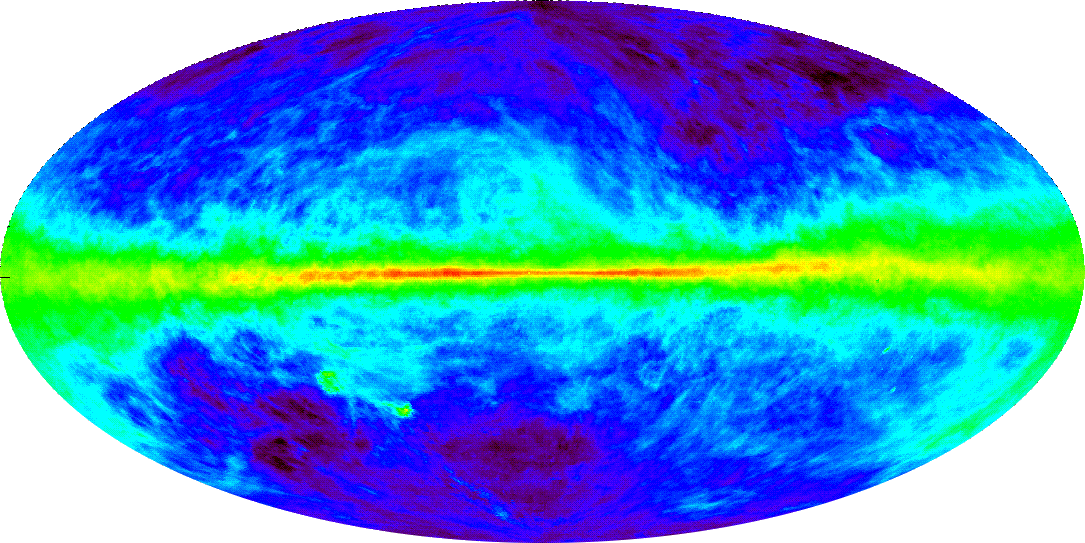
\includegraphics[width=1\linewidth]{Images/21.png}
	\caption{Εκπομπή του \ce{HI} στα 21.1 cm (Kalberla et al., 2005)%\cite{kalberla_2005}.
		H εκπομπή της γραμμής $21.1 \, cm$ στα ραδιοκύματα που οφείλεται στη μετάπτωση αντιστροφής του spin του πρωτονίου και του ηλεκτρονίου στη βασική κατάσταση του ατόμου του Υδρογόνου. Η ενεργειακή διαφορά των καταστάσεων είναι 
		$h \nu=\SI{6e-6}{eV}$, η οποία αντιστοιχεί σε μήκος κύματος \SI{21}{cm}.}
\end{marginfigure}

\begin{marginfigure}
	\label{fig:Ha}
	\centering
	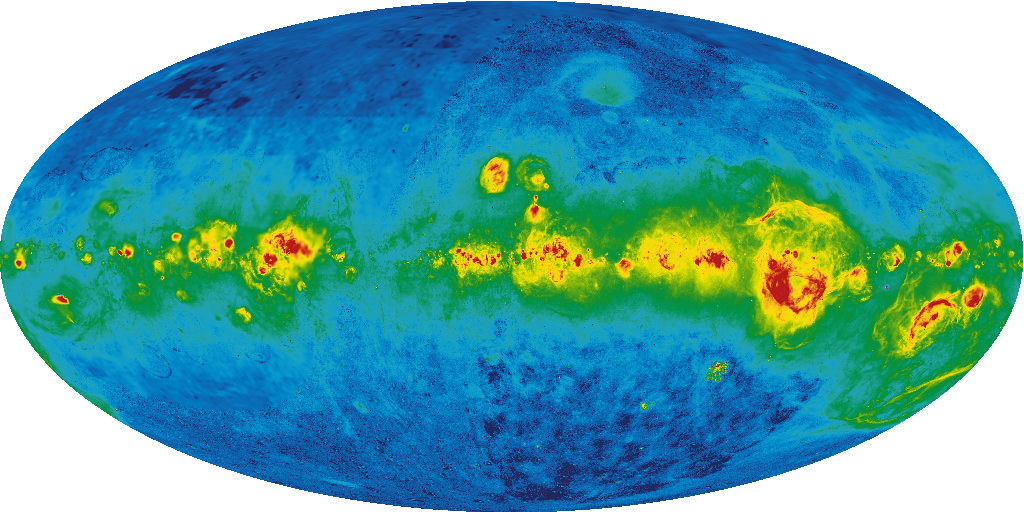
\includegraphics[width=1\linewidth]{Images/Ha.png}
	\caption{Εκπομπή Ha από συνδυασμό τριών διαφορετικών παρατηρήσεων (WHAM - VTSS - SHASSA) \cite{finkbeiner_2003}. Η εκπομπή Ha (\SI{656.28}{nm}) προέρχεται από την επανασύνδεση ιονισμένων ατόμων υδρογόνου κοντά σε θερμούς αστέρες O και B (\ce{HII} Regions).}
\end{marginfigure}


\paragraph{Μεσοαστρικό Αέριο} 
Το Μεσοαστρικό Αέριο παρατηρείται σε νεφελώδη μορφή και αποτελείται κυρίως (περίπου το 90\%) από υδρογόνο σε ατομική \ce{(H)}, ιονισμένη \ce{(HII)} και μοριακή \ce{(H2)} κατάσταση. Δεύτερο σε αναλογία είναι το Ήλιο \ce{(He)} (περίπου 9\%) ενώ το υπόλοιπο 1\% είναι βαρύτερα στοιχεία (\ce{C},\ce{O},\ce{Ne},\ce{Mg},\ce{Fe}, κ.α.) και μόρια (\ce{CO},\ce{CS}, κ.α.).


\paragraph{Μεσοαστρική Σκόνη}
%\begin{figure}[h]
%	\centering
%	\includegraphics[width=\medpage]{images/dust_emission_planck.png}
%	\caption{Εκπομπή της σκόνης του Γαλαξία μας όπως τη χαρτογράφησε το Planck.\cite{planck_2014}}
%\end{figure}

Η Μεσοαστρική Σκόνη αποτελείται κυρίως από άνθρακα και πυρίτιο σε ενώσεις με Υδρογόνο, Οξυγόνο, Μαγνήσιο και Σίδηρο ενώ το μέγεθος των κόκκων της σκόνης κυμαίνεται από \SI{0.01}{\micro\meter} έως \SI{1}{\micro\meter} ακολουθώντας μια κατανομή δύναμης όπου τα μικρότερα μεγέθη είναι πολυπληθέστερα από τα μεγαλύτερα. 
Η Μεσοαστρική Σκόνη παρατηρείται στις σπείρες του Γαλαξία μας (αλλά και σε άλλους γαλαξίες) με τη χαρακτηριστική μορφή τεράστιων σκοτεινών "δρόμων" λόγω της επισκότισης των όπισθεν αστέρων που προκύπτει από την απορρόφηση και σκέδαση του ορατού φωτός.


\section{Φάσεις και χαρακτηριστικά της Μεσοαστρικής Ύλης}
Η Μεσοαστρική Ύλη (ISM) απαντάται σε τρεις φάσεις με διαφορετικά φυσικά και χημικά χαρακτηριστικά: 
\footnote{Για τα χημικά χαρακτηριστικά αναφερόμαστε στή σύνθεση των μορίων και στην αναλογία των στοιχείων. Στα φυσικά χαρακτηριστικά αναφερόμαστε στη πυκνότητα και τη θερμοκρασία της Ύλης} 
τη \textbf{ψυχρή}, με θερμοκρασίες κάτω των \SI{100}{\kelvin},
 πυκνότητα \SIrange{30}{50}{cm^{-3}} και ποσοστό ιονισμού κάτω του 0.1\%, που αποτελείται από μοριακό και ατομικό αέριο Υδρογόνου και σκόνη, τη \textbf{θερμή}, με θερμοκρασίες της τάξης των \SIrange{1e3}{1e4}{K}, πυκνότητες \SI{0.3}{cm^{-3}}, που αποτελείται από ατομικό και ιονισμένο άεριο Υδρογόνο (ποσοστό ιονισμού 2-20\%) και την \textbf{υπέρθερμη} που οφείλεται σε κρουστικά κύματα εκρήξεων supernova και αστρικών ανέμων με θερμοκρασίες τάξης \SI{1e6}{K} και πυκνότητες μικρότερες των \SI{0.01}{cm^{-3}}.

\marginpar{
	\begin{table}[H]
		\caption{Χαρακτηριστικά \newline της μεσοαστρικής ύλης}
		\label{tab:ISM}
		\begin{tabular}{p{2.5cm} c  c  c }
			\toprule
			\multirow{2}{*}{Κατηγορία}  & Θερμοκρασία & Πυκνότητα   \\ 
			& \si{(K)} & \si{(cm^{-1})}  \\
			\midrule
			Μοριακά Νέφη & 10-50 & \num{>1e3} \\
			Ψυχρά Νέφη \ce{HI}  & \num{100} & \num{30} \\
			Θερμό \ce{HI}  & \num{1e3} & \num{0.1} \\
			Θερμό \ce{HII}  & \num{1e4} & \num{1e-2} \\
			Περιοχές \ce{HII} &  \num{1e4} & \num{>100} \\
			Υπέρθερμο Ιονισμένο αέριο &  \numrange{1e6}{1e7} & \num{1e-3} \\
			\bottomrule
		\end{tabular}
	\end{table}
}




%\subsection{Παρατηρήσεις της Μεσοαστρικής Ύλης}
%Η παρατήρηση και μελέτη της Μεσοαστρικής Ύλης ποικίλει αναλόγως τη φάση στην οποία βρίσκεται.
%\subparagraph{Εκπομπή 21.1 cm}
%%\begin{figure}[h]
%%	\label{fig:21}
%%	\centering
%%	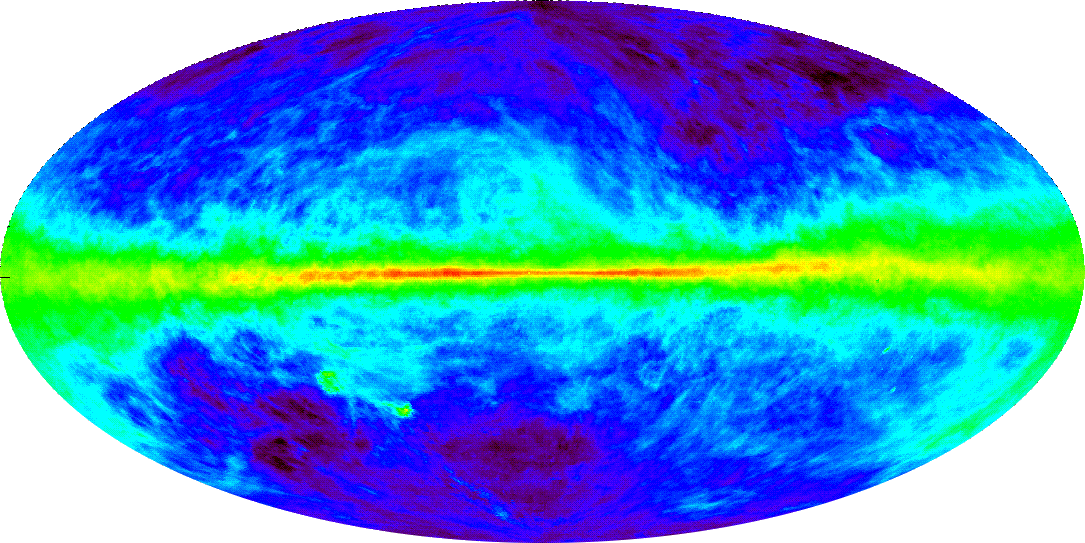
\includegraphics[width=\medpage]{images/21.png}
%%	\caption{Εκπομπή του \ce{HI} στα 21.1 cm (Kalberla et al., 2005)\cite{kalberla_2005}}
%%\end{figure}
%
%H καλύτερη μέχρι σήμερα δυνατή μέθοδος για την παρατήρηση του \textbf{Ουδέτερου Υδρογόνου \ce{H I}} είναι η εκπομπή της γραμμής $21.1 \, cm$ στα ραδιοκύματα που οφείλεται στη μετάπτωση αντιστροφής του spin του πρωτονίου και του ηλεκτρονίου στη βασική κατάσταση του ατόμου του Υδρογόνου. Η ενεργειακή διαφορά των καταστάσεων με συνολικό spin $F=1$ \textbf{(τα spin $p^+$ και $e^-$ είναι παράλληλα)} και $F=0$ \textbf{(τα spin $p^+$ και $e^-$ είναι άντιπαράλληλα)} είναι $h \nu=6\times 10^{-6} \, eV$, η οποία αντιστοιχεί στη γραμμή των 21 cm.
%Ο συντελεστής Einstein για την αυθόρμητη εκπομπή είναι $A_{10} \simeq 3\times 10^{-15}s^{-1}$ που αντιστοιχεί σε μια χρονική κλίμακα των $10^7$ ετών στην οποία παραμένει ένα διεγερμένο άτομο Υδρογόνου μέχρι να αποδιεγερθεί αυθόρμητα εκπέμποντας το παρατηρούμενο φωτόνιο. Ο πολύ μικρός αυτός ρυθμός εκπομπής αντιπαραβάλλεται εν τέλει από τη τεράστια ποσότητα του ατομικού υδρογόνου έτσι ώστε στατιστικά η γραμμή να είναι παρατηρήσιμη.
%
%\subparagraph{Εκπομπή \ce{H\alpha}}
%Κοντά σε αστέρες μεγάλης μάζας (φασματικού τύπου O και B) λόγω των φωτονίων υψηλής ενέργειας (μεγαλύτερες από το όριο Lyman) το αέριο υδρογόνο ιονίζεται. Οι περιοχές αυτές, ονομάζονται και Περιοχές HII, θα τις εξετάσουμε αναλυτικότερα στη παράγραφο~(\ref{par:HII regions}), και παρουσιάζουν έντονη εκπομπή ακτινοβολίας στη γραμμή Ha $(656.28\ nm)$ λόγω της επανασύνδεσης των ιονισμένων ατόμων.

%\begin{figure}[h]
%	\label{fig:Ha}
%	\centering
%	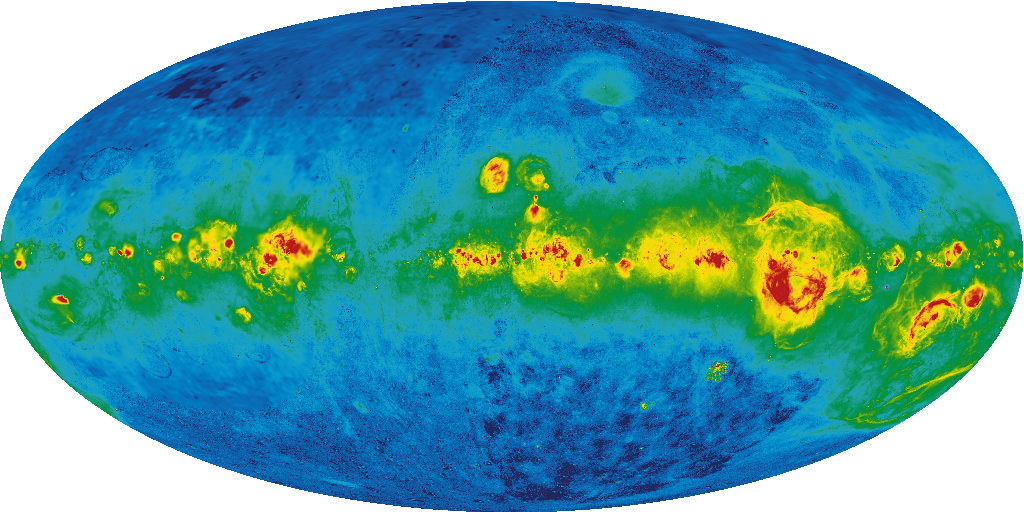
\includegraphics[width=\medpage]{images/Ha.png}
%	\caption{Εκπομπή Ha από συνδυασμό τριών διαφορετικών παρατηρήσεων (WHAM - VTSS - SHASSA) \cite{finkbeiner_2003}}
%\end{figure}
%

%===================================================================
%===================================================================
%===================================================================

\section{Μοριακά Νέφη}
%Οι πιο ενδιαφέρουσες, από τη σκοπιά της δημιουργίας αστέρων, περιοχές του Μεσοαστρικού Υλικού είναι τα Μοριακά Νέφη (Molecular Clouds).
Τα Μοριακά Νέφη είναι περιοχές όπου ψυχρή μεσοαστρική ύλη έχει πυκνότητες ικανοποιητικά μεγαλύτερες από τη μέση πυκνότητα του μεσοαστρικού υλικού έτσι η ιδιοβαρύτητα του νέφους να παίζει σημαντικό ρόλο στη δυναμική του. Καθώς το μοριακό νέφος καταρρέει, κατακρημνίζεται σε όλο και πιο συμπυκνωμένες δομές έως ότου η πυκνότητα και η μάζα σε μια τέτοια περιοχή είναι αρκετή ώστε να γεννηθούν νέοι αστέρες.   

\begin{marginfigure}
	\label{fig:CO}
	\centering
	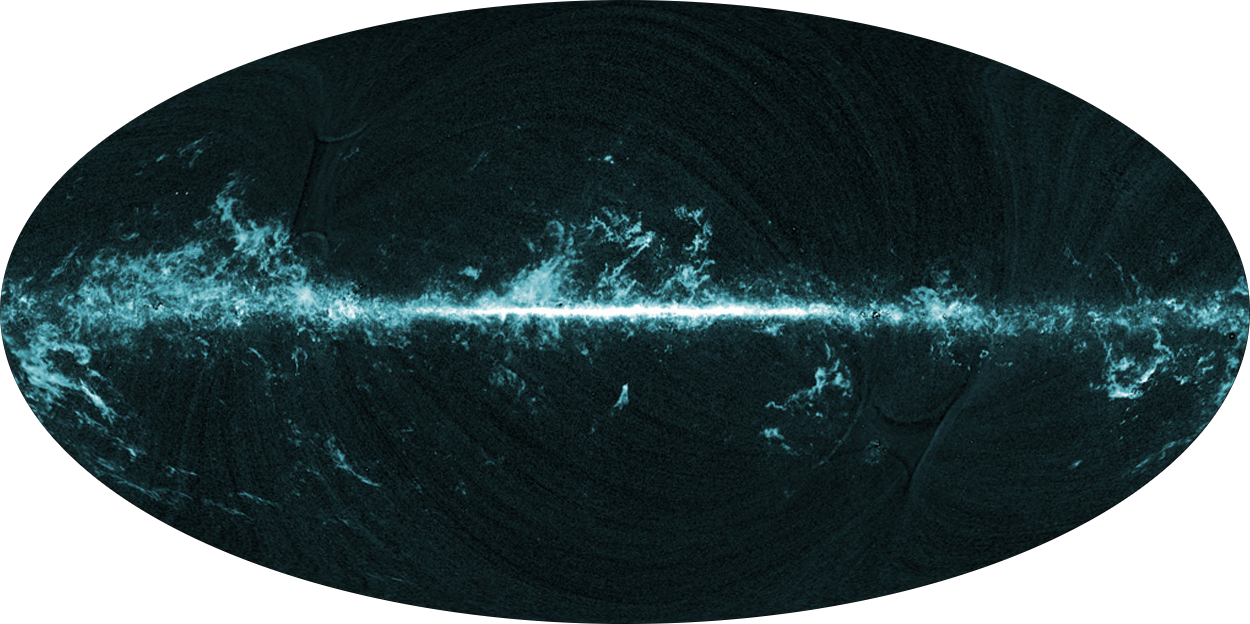
\includegraphics[width=1\linewidth]{Images/CO.png}
	\caption{Εκπομπή CO όπως τη χαρτογράφησε το Planck.\cite{planck_2014}.
		\newline
		Το \ce{H2} είναι ένα πλήρως συμμετρικό μόριο επομένως δεν έχει μόνιμη διπολική ροπή. Αυτό έχει σαν συνέπεια η διέγερση του να είναι σε θερμοκρασίες τις τάξεις των \SI{500}{K}. Άρα για τις τυπικές θερμοκρασίες των μοριακών νεφών $10-50\ K$ είναι αδύνατον να το παρατηρήσουμε άμεσα.
		\newline
		Ο εναλλακτικός τρόπος παρατήρησης του \ce{H2} είναι εμμέσως μέσω της εκπομπής διαφορετικών μορίων που είναι πιο "ευαίσθητα" στις χαμηλές θερμοκρασίες, όπως του \ce{CO} που είναι το δεύτερο σε αναλογία μόριο στο Σύμπαν και έχει μόνιμη διπολική ροπή (άρα έχουμε περιστροφικές ενεργειακές μεταβάσεις) πράγμα του επιτρέπει να εκπέμπει σημαντικά στο ραδιοφωνικό φάσμα.. 
		\newline
		H χαμηλότερη μετάβαση αντιστοιχεί σε θερμοκρασία \SI{5.5}{K} και αποδίδει ένα ραδιοφωνικό φωτόνιο στα \SI{2.6}{mm}.
	}
	%
	%Ο κύριος μηχανισμός διέγερσης ενός μορίου \ce{CO} στη $J=1$ είναι μέσω της σύγκρουσης του με ένα μόριο \ce{H2}. Αφού διεγερθεί η αποδιέγερση του μπορεί να γίνει είτε εκπέμποντας ένα φωτόνιο στα \SI{2.6}{mm} σε περιοχές με χαμηλή συνολική πυκνότητα είτε μεταφέροντας την ενέργεια του σε ξανά σε ένα μόριο \ce{H2} χωρίς να εκπεμφθεί φωτόνιο σε περιοχές με μεγάλη συνολική πυκνότητα.
	
\end{marginfigure}

Όπως φαίνεται και από το όνομα τους, τα Μοριακά Νέφη αποτελούνται κυρίως από μοριακό Υδρογόνο \ce{H2}. Στο γαλαξία μας πάνω από το 80\% του μοριακού Υδρογόνου βρίσκεται σε μοριακά νέφη κατανεμημένα πάνω στις σπείρες του δίσκου αλλά κυρίως σε ένα δακτύλιο ακτίνας 3 με 5 kpc από το κέντρο του γαλαξία \cite{rathborne_2009}.  Από παρατηρήσεις στο \ce{CO} τα μοριακά νέφη δείχνουν να έχουν μάζες που κυμαίνονται από \SIrange{1e3}{1e6}{M_\odot} με μια κατανομή νόμου δύναμης $-1.6$. \cite{stahlern_2004}

Για να δημιουργηθεί το Μοριακό Υδρογόνο καταλυτικό ρόλο παίζει η μεσοαστρική σκόνη.  Όταν δύο άτομα Υδρογόνου ενώνονται και δημιουργούν ένα μόριο \ce{H2} αυτό κερδίζει ενέργεια η οποία όμως δεν μπορεί να αποδοθεί στο περιβάλλον με αποτέλεσμα το μόριο να διασπάται. Παρολαυτά αν η διαδικασία αυτή γίνει πάνω σε έναν κόκκο σκόνης, τότε αυτός λειτουργεί καταλυτικά απορροφώντας το πλεόνασμα ενέργειας και το μόριο παραμένει σταθερό. Έτσι το ουδέτερο Υδρογόνο λειτουργεί σαν καύσιμο που τροφοδοτεί τις πυκνότερες περιοχές του μοριακού Υδρογόνου.

Ένα τυπικό μοριακό νέφος επιβιώνει για \SI{3e7}{yrs} πριν καταστραφεί από τους βίαιους αστρικούς ανέμους των αστέρων τύπου O και B που έχουν δημιουργηθεί στο εσωτερικό του. Κατά τη διάρκεια της ζωής του το νέφος αποδίδει τελικά ένα 3\% της μάζας του σε αστέρες. Έτσι για παράδειγμα αν θεωρήσουμε μια τιμή της συνολικής μάζας του μοριακού \ce{H2} στο Γαλαξιακό δίσκο \SI{2e9}{M_\odot} βρίσκουμε ότι ο ρυθμός δημιουργίας αστέρων (SFR) για το Γαλαξία μας είναι περίπου \SI{2}{M_\odot} ανά έτος.  


\begin{table}
	\caption{Χαρακτηριστικά και διαφορετικοί τύποι Μοριακών Νεφών}
	\label{tab:MCtypes}
	\begin{tabular}{l c c c c}
		\toprule
		\multirow{2}{*}{Κατηγορία} & Μέση ακτίνα &  Θερμοκρασία & Πυκνότητα \ce{H2} & Μάζα \\ 
		& \si{(pc)} & \si{(K)} & \si{(cm^{-3})} & \si{(M_\odot)} \\
		\midrule
		Γιγαντιαίο Μοριακό Νέφος & \num{20} & \num{15} & \num{100} & \num{1e5} \\
		Μοριακό Νέφος & $5$ & $10$ & $300$ & $10^4$\\
		clump & $2$ & $10$ & $10^3$ & $10^3$\\
		Πυρήνας Νέφους & $0.08$ & $10$ & $10^5$ & $10$\\
		\bottomrule
	\end{tabular}
\end{table}


%\subsection{Ενεργειακή ισορροπία στα Μοριακά Νέφη}
%Όπως αναφέραμε γενικότερα στη παράγραφο~(\ref{par:EnergyBalance}) η θερμοκρασία ενός νέφους είναι αποτέλεσμα στης ενεργειακής ισορροπίας μεταξύ των μηχανισμών θέρμανσης και ψύξης. Για τα Μοριακά Νέφη συγκεκριμένα η θέρμανση είναι αποτέλεσμα της θερμότητας που παρέχεται από κοντινά άστρα ή μέσω της κοσμικής ακτινοβολίας, ενώ η ψύξη επιτυγχάνεται μέσω διαδικασιών απορρόφησης και κρούσης με τα σωματίδια της σκόνης ή του αερίου.
%Η ενέργεια τελικά αποδίδεται μέσω της υπέρυθρης ακτινοβολίας η οποία οφείλεται στην απορρόφηση και την εκπομπή των φωτονίων από το περιβάλλοντα αέριο και σκόνη.
%

\section{Ενεργειακή ισορροπία}
\label{par:EnergyBalance}
Η κινητική θερμοκρασία \footnote{Το ψυχρό μεσοαστρικό αέριο λόγω της γενικά χαμηλής του πυκνότητας δεν βρίσκεται σε θερμοδυναμική ισορροπία. Επομένως όταν μιλάμε για θερμοκρασία αναφερόμαστε στη κινητική του θερμοκρασία.\cite[p. 28]{spitzer_1998}} της Μεσοαστρικής Ύλης κυμαίνεται σε ένα εύρος τιμών 6 τάξεων μεγέθους όπως παρατηρούμε και από τον πίνακα~\ref{tab:ISM}. Για να περιγράψουμε και να μοντελοποιήσουμε την ενεργειακή ισορροπία στη Μεσοαστρική Ύλη και άρα να εξηγήσουμε και τις παρατηρούμενες θερμοκρασίες θα πρέπει να υπολογίσουμε τις διαδικασίες θέρμανσης και ψύξης. 
%Ενώ η κύρια διαδικασία ψύξης είναι η εκπομπή ακτινοβολίας είτε μέσω αυθόρμητης αποδιέγερσης ή αποδιέγερσης λόγω κρούσης, για τη θέρμανση έχουμε μια πληθώρα διαδικασιών οι οποίες μπορούν να ταξινομηθούν σε 3 κατηγορίες:
%
%\begin{itemize}
%	\item θέρμανση από πεδία ακτινοβολίας: φωτοηλεκτρική απορρόφηση σε ουδέτερα στοιχεία, φωτοδιάσπαση στα μόρια, φωτοιονισμός.
%	\item θέρμανση μέσω συγκρούσεων: από τυρβώδες ροές, κρουστικά κύματα καταλοίπων supernova και κοσμικής ακτινοβολίας.
%	\item θερμική ανταλλαγή μεταξύ της σκόνης και νεφών αερίου, αλληλεπίδραση ιονισμένου αερίου με μαγνητικά πεδία, βαρυτική κατάρρευση. 
%\end{itemize}

%=======ΦΩΤΗΣ==================
Ο πιο γενικός διαχωρισμός των μηχανισμών θέρμανσης και ψύξης αφορά τις διαδικασίες που έχουν να κάνουν με θέρμανση λόγω φώτο-ιονισμού και διαδικασίες ψύξης λόγω διέγερσης από αλληλεπίδραση μεταξύ σωματιδίων. Παρακάτω θα παρουσιαστεί μια διαισθητική εικόνα των διαδικασιών αυτών.
\begin{itemize}
	\item \textbf{Φώτο-ιονισμός ουδέτερων ατόμων} \\
	Ένα φωτόνιο προσπίπτει σε ένα ουδέτερο άτομο επάγοντας τον ιονισμό του. Έχουμε λοιπόν ένα ελεύθερο ηλεκτρόνιο με ενέργεια $E$ το οποίο μέσω συγκρούσεων με άλλα ουδέτερα σωμάτια του αερίου μεταφέρει ενέργεια στο αέριο, θερμαίνοντας το. Ωστόσο, λόγω επανασύνδεσης (recombination) η αποδιδόμενη ενέργεια είναι μικρότερη απο την αρχική ενέργεια του ηλεκτρονίου.
	\item \textbf{Αλληλεπιδράσεις μεταξύ σωματιδίων} \\ Ελεύθερα σωματίδια αλληλεπιδρούν μέσω κρούσεων επάγοντας μεταβάσεις σε διεγερμένες ενεργειακές στάθμες. Κατά τις συνεπακόλουθες μεταβάσεις στην βασική κατάσταση εκπέμπονται φωτόνια, τα οποία εφόσον διαφύγουν από την περιοχή αντιστοιχούν σε απώλεια ενέργειας.
	Ακολουθεί μια αυστηρότερη περιγραφή των παραπάνω διεργασιών.
	% θελει πιο ομορφη περιγραφη, μοιαζει με κείμενο πενταχρονου
\end{itemize}
\subsection{Θερμοδυναμική περιγραφή}
Ξεκινάμε από τον πρώτο νόμο τις θερμοδυναμικής:
\begin{equation}
dE = \bar{d}Q - dW
\end{equation}
Όπου $dE$ η μεταβολή της εσωτερικής ενέργειας, $\bar{d}Q$ η θερμότητα που απορρόφησε το σύστημα και $dW$ το έργο που έγινε από το σύστημα.

% Για ημιστατικό σύστημα έχουμε οτι $\bar{d}Q = TdS$, $dS$ το διαφορικό της εντροπίας και επίσης απο τον ορισμό του έργου, $dW=pdV$ όπου $dV$ η μεταβολή του όγκου του συστήματος και $p$ η πίεση.
%
%\begin{equation}
%TdS =dE +pdV
%\end{equation}
Για ιδανικά αέρια, η εσωτερική ενέργεια εξαρτάται μόνο απο τη θερμοκρασία και η καταστατική εξίσωση γράφεται ως: $p=nk_bT$, όπου $k_b$ η σταθερά του Boltzmann και $n$ η αριθμητική πυκνότητα του αερίου. Ακολούθως, 
χρησιμοποιώντας το ότι η εσωτερική ενέργεια μονατομικού ιδανικού αερίου είναι $E = \frac{3}{2}NkT$ η απορροφούμενη θερμότητα ανά μονάδα όγκου είναι:

\begin{equation}
\frac{dQ}{V}=nd\left(\frac{3}{2}kT \right)-kTdn
\end{equation}

Στη γενικότητα, οι διαδικασίες θέρμανσης και ψύξης εξαρτώνται από τον χρόνο και η ολική ενέργεια ανά μονάδα όγκου ανά μονάδα χρόνου ισούται με:

\begin{equation}
\label{eq:CoolingHeating}
\Delta = n\frac{d}{dt}\left(\frac{3}{2}kT \right)-kT\frac{dn}{dt}
\end{equation}
\marginpar{
	Στην σχέση \ref{eq:CoolingHeating} αγνοήσαμε τη θερμική αγωγιμότητα η οποία δεν παίζει ιδιαίτερο ρόλο στις τυπικές θερμοκρασίες του μεοαστρικού υλικού $T< 2\cdot 10^{4}K$. Γενικά θα έπρεπε να προσθέσουμε στο αριστερό μέλος την ποσότητα $\nabla \cdot (K\nabla T) $ όπου $K$ η θερμική αγωγιμότητα. Εδώ θα πρέπει να σημειωθεί ότι σε περιοχές υψηλών θερμοκρασιών, η παρουσία μαγνητικών πεδίων επηρεάζει επιπλέον την θερμική αγωγιμότητα.
}

Έστω τώρα ότι η θερμότητα ανά μονάδα όγκου και χρόνου που προστίθεται στο αέριο από την αλληλεπίδραση των σωματιδίων $\xi,n$ είναι $\Gamma_{\xi \eta}$ και όμοια, η συνεισφορά των αλληλεπιδράσεων αυτών στην ψύξη είναι $\Lambda_{\xi \eta} $. Ορίζουμε τις συναρτήσεις ψύξης (cooling function) και θέρμανσης (heating function) ως:

\begin{equation}
\Lambda = \sum_{\xi \eta}\Lambda_{\xi \eta}
\label{thermFunction}
\end{equation}

\begin{equation}
\Gamma = \sum_{\xi \eta}\Gamma_{\xi \eta}
\end{equation}
Συνεπώς έχουμε ότι:
\begin{equation}
\Delta = \Gamma -\Lambda
\end{equation}
Μπορούμε να δούμε ότι αν η αριθμητική πυκνότητα και η θερμοκρασία δεν μεταβάλλονται με τον χρόνο ισχύει ότι 
\begin{equation}
\Delta = 0 \Rightarrow \Gamma = \Lambda 
\end{equation}
Με βάση τη τελευταία σχέση μπορούμε να ορίσουμε τη \emph{θερμοκρασία ισορροπίας}. Για τον ορισμό της τελευταίας χρειάζεται να γνωρίζουμε όλους τους μηχανισμούς θέρμανσης και ψύξης του αερίου. Στο υπόλοιπο κείμενο θα θεωρήσουμε οτι το αέριο βρίσκεται στη θερμοκρασία σταθερής κατάστασης εκτός και αν αναφέρεται κάτι διαφορετικό. Εν συνεχεία θα παρουσιάσουμε τις συναρτησεις ψύξης/θέρμανσης για διάφορες φυσικές διαδικασίες.

% % % % % % % 
%Εδώ πρέπει να συζητηθεί η %χρονική κλίμακα των %transient φαινομένων.
\subsection{Μηχανισμοί Θέρμανσης}
\subsubsection{Κοσμική ακτινοβολία}
Ένας πολύ σημαντικός μηχανισμός θέρμανσης της μεοαστρικής ύλης και κατα συνέπεια και των μοριακών νεφών είναι η κοσμική ακτινοβολία. Η κοσμική ακτινοβολία αποτελείτε επί το πλείστον από σχετικιστικά πρωτόνια μαζί με λιγότερα βαρύτερα στοιχεία ή ηλεκτρόνια. Η ενεργειακή κατανομή των κοσμικών αυτών σωματιδίων κυμαίνεται από ενέργειες των \SIrange{10}{1e14}{MeV} με κατανομή νόμου δύναμης $\Phi _\mathtt{CR}(E)\sim E^{-2.7}$ (για τη ροή).

\todo{φωτο κατανομη κοσμικης ακτινοβολιας}
%\paragraph{Αλληλεπίδραση Κοσμικής ακτινοβολίας με μοριακό αέριο}
Κατά την αλληλεπίδραση ενός πρωτονίου της κοσμικής ακτινοβολίας με το μοριακό υδρογόνο ενός μοριακού νέφους είτε το \ce{H2} θα διεγερθεί και θα διασπαστεί σε δύο Υδρογόνα είτε θα έχουμε απευθείας ιονισμό. Ξεκινώντας από τον ιονισμό έχουμε την αντίδραση:
\begin{equation}
\ce{p^+ +H2 -> H2 ^+ +e^- +p^+}
\end{equation}
Καθώς το ηλεκτρόνιο που διαφεύγει αλληλεπιδρά με τα γειτονικά μοριακά υδρογόνα θερμαίνει το αέριο με ρυθμό
\begin{equation}
\Gamma _\mathtt{CR} (\ce{H2}) =\zeta (\ce{H2})n_{\ce{H2}} \Delta E (\ce{H2})
\end{equation}
όπου $\zeta (\ce{H2})$ είναι ο ρυθμός ιονισμού ενός μορίου \ce{H2}, $n_{\ce{H2}}$ η αριθμητική πυκνότητα του μοριακού υδρογόνου και $\Delta E (\ce{H2})$ η θερμική ενέργεια που προσδίδεται στο αέριο σε κάθε ιονισμό. Η ενέργεια αυτή εξαρτάται από την ενέργεια του κοσμικού πρωτονίου. Πρωτόνια με ενέργεια μεγαλύτερη του \SI{1}{GeV} διεγείρουν το πυρήνα με αποτέλεσμα την εκπομπή ακτίνων γ και δεν εναποθέτουν ενέργεια στο αέριο. Παίρνοντας μια τυπική για το πρωτόνιο τιμή των \SI{10}{MeV} η ενέργεια που αποδίδεται στο ηλεκτρόνιο είναι \SI{30}{eV}. 

Το ηλεκτρόνιο τώρα μπορεί είτε να ιονίσει περαιτέρω το μοριακό αέριο μέσω της
\begin{equation}
\ce{e^- + H2 -> H2^+ + e^- + e^-}
\end{equation}
η οποία δεν προσδίδει θέρμανση αλλά εμπλουτίζει το χώρο με περισσότερο ενεργητικά ηλεκτρόνια ή να θερμάνει τελικά το αέριο μέσω της διάσπασης του μορίου
\begin{equation}
\ce{e^- + H2 -> H + H + e^-}
\end{equation} 
Κάνοντας το λεπτομερή υπολογισμό μέσω του δικτύου όλων τα πιθανών σεναρίων βρίσκουμε ότι η ενεργειακή ενέργεια ανά ιονισμό είναι $\Delta E (\ce{H2}) = \SI{7}{eV}$. Η τιμή αυτή δεν εξαρτάται σημαντικά από την ενέργεια του κοσμικού πρωτονίου, ενδεικτικά η τιμή του $\Delta E (\ce{H2})$ για ενέργειες πρωτονίων \SIrange{1}{100}{MeV} κυμαίνεται αντίστοιχα στα \SIrange{6.3}{7.6}{eV}.

Στη περίπτωση της αλληλεπίδρασης της κοσμικής ακτινοβολίας με ουδέτερο Υδρογόνο ο ιονισμός πραγματοποιείται μέσω της:
\begin{equation}
\ce{p^+ + H -> H^+ + e^- + p^+}
\end{equation}
όπου το ηλεκτρόνιο τώρα δραπετεύει με ενέργεια στα \SI{35}{eV} συνεισφέροντας με ρυθμό θέρμανσης αντίστοιχα με πριν
\begin{equation}
\Gamma _\mathtt{CR} (\ce{HI}) =\zeta (\ce{HI})n_{\ce{HI}} \Delta E (\ce{HI})
\end{equation}

Η ενέργεια του ηλεκτρονίου είναι όμως αρκετά υψηλή ώστε για να θερμάνει το αέριο, εφόσον κάθε αλληλεπίδραση έχει αποτέλεσμα νέους ιονισμούς. Τελικά η θέρμανση θα ξεκινήσει όταν το ηλεκτρόνιο αποχτήσει ενέργεια κάτω από \SI{10.2}{eV} η οποία αντιστοιχεί στη πρώτη διεγερμένη στάθμη του υδρογόνου ($n=2$). Έπειτα από αριθμητικούς υπολογισμούς η ενέργεια ανά ιονισμό $\Delta E (\ce{HI})$ υπολογίζεται στα \SI{6}{eV}.

Για τον τελικό υπολογισμό 



\paragraph{Φώτο-ιονισμός ουδέτερων ατόμων}
Ένας από τους πιο σημαντικούς μηχανισμούς θέρμανσης του μεσοαστρικού αερίου προέρχεται από το φώτο-ιονισμό των ουδέτερων ατόμων. Σε αυτή τη διαδικασία ένα φωτόνιο με ενέργεια $h \nu$ ιονίζει ένα ηλεκτρόνιο δίνοντας του πλεόνασμα ενέργειας $E$. Το ηλεκτρόνιο μπορεί να συγκρουστεί με άλλα σωματίδια αναδιανέμοντας την ενέργεια αυτή υπό τη μορφή θέρμανσης

Ο ρυθμός φώτο-ιονισμού (ή πιθανότητα φώτο-ιονισμού ανά μονάδα χρόνου), $\beta_{\mathtt{j,ph}}$ μπορεί να συσχετιστεί με την ενεργό διατομή $\sigma_{\nu,ph}$ των bound-free μεταβάσεων. Αρχικά θα χρειαστούμε την πιθανότητα της bound-bound μετάβασης απο την στάθμη j στην στάθμη k, $\beta_{jk}$. Η ενέργεια ανά μονάδα όγκου και ανα μονάδα χρόνου είναι, \cite{RybickiLightman}, 
$
U_{\nu} = \frac{1}{c}\int I_{\nu}d\Omega
$
, όπου $I_{\nu}$ η ειδική ένταση της ακτινοβολίας.
Η απορροφούμενη ενέργεια θα πρέπει να είναι ανάλογη του γινομένου του συντελεστή απορρόφησης $k_{\nu}$ με την $U_{\nu}$. Ο ρυθμός των μεταβάσεων $j \rightarrow k$ ανα μονάδα όγκου είναι:
\begin{equation}
R_{tr} = \int\frac{cU_{\nu}k_{\nu}}{h\nu}d\nu
\end{equation}
Πολλαπλασιάσαμε με την ταχύτητα του φωτός για διαστατικούς λόγους καθώς ο συντελεστής απορρόφησης έχει μονάδες $cm^{-1}$.
Η ζητούμενη πιθανότητα ανα μονάδα χρόνου των μεταβάσεων θα είναι ο ρυθμός των μεταβάσεων προς την αριθμητική πυκνότητα της αρχικής στάθμης j:

\begin{equation}
\beta_{jk}=\frac{1}{\nu_{j}}\int \frac{cU_{\nu}k_{\nu}}{h\nu}d\nu
\end{equation}
Ακόμα ισχύει οτι $k_{\nu}=n_{j}\sigma$ συνεπώς:
\begin{equation}
\beta_{jk}=\int \frac{cU_{\nu}\sigma}{h\nu}d\nu
\end{equation}
Όμοια για το φωτο-ιονισμό έχουμε:
\begin{equation}
\beta_{j,ph}=\int_{\nu_{0}}^{\infty} \frac{cU_{\nu}\sigma_{ph}}{h\nu}d\nu
\end{equation}
Όπου η ολοκλήρωση αρχίζει απο την κρίσιμη συχνότητα $ \nu_{0}$, κάτω απο την οποία δεν επαρκεί η ενέργεια του φωτονίου ωστε να γίνει η μετάβαση.

Η απαίτηση της ισορροπίας μεταξύ ιοντισμών και επανασύνδεσης δίνει την ακόλουθη ισότητα:
\begin{equation}
\sum_{j}n_{j}(X^{r})\beta_{j,ph} = \sum_{j}n(X^{r+1})n_{e}a_{j}
\end{equation}
όπου $n_{j}(X^{r}), \ n(X^{r+1})$ οι αριθμητικές πυκνότητες των ιόντων $X^{r}$ και $X^{r+1}$ αντίστοιχα, ενώ $\beta_{j,ph}, \ a_{j}$ οι ρυθμοί φωτο-ιονισμών και επανασύνδεσης. Η τελευταία εξίσωση αναφέρεται ως εξίσωση ισορροπίας ιοντισμών (ionization equilibrium). Εν συνεχεία θα εξαχθεί η συνάρτηση θέρμανσης. Ξεκινάμε απο την εξ. \ref{thermFunction} θεωρόντας αλληλεπιδράσεις μεταξύ ηλεκτρονίων και ιόντων. 

\begin{equation}
\Gamma_{ei} = \sum_{j}\left( n_{j}(X^{r})\beta_{j,ph}-\beta_{j,ph}E_{loss}\right)
\end{equation}
Όπου $E_{loss}$ ειναι η ενέργεια του φωτονίου που προκύπτει απο την επανασύνδεση. Η παραπάνω έκφραση είναι συνάρτηση της ταχύτητας των ηλεκτρονίων. Πρέπει λοιπον να ληφθεί η μέση τιμή της.
\begin{equation}
\Gamma_{ei} = \int\sum_{j}\left( n_{j}(X^{r})\beta_{j,ph}-\beta_{j,ph}E_{loss}\right)f(\vec{u})d^{3}\vec{u}
\end{equation}
Υποθέτουμε ότι οι ταχύτητες τών ηλεκτρονίων ακολουθούν κατανομή Maxwell. Αντίκαθιστούμε το $n(X^{r+1})$ με την αριθμητική πυκνότητα των ιονισμένων ατόμων, $n_{i}$ και $a_{j} = [\sigma_{cj}\nu] $. 
\begin{equation}
\Gamma_{ei} = n_{e}n_{i}\sum_{j}\left[<\sigma_{cj}\nu>\bar{E_{2}}-<\sigma_{cj}\nu E_{loss}>\right]
\end{equation}
Όπου $\bar{E_{2}}$ η μέση ενέργεια φωτοιονισμού.  Ισχύει ότι $a = \sum_{j}a_{j}$ για τον συντελεστή επανασύνδεσης για το ενεργειακό επίπεδο j.
Υποθέτοντας επιπλέον οτι οι φωτοιονισμοί προκύπτουν απο την βασική κατάσταση έχουμε:

\begin{equation}
\Gamma_{ei} = n_{e}n_{i}\left(a\bar{E_{2}}-\frac{1}{2}m_{e}\sum_{j}<\sigma_{cj}u^3> \right)
\end{equation}
Όπου αντικαταστήσαμε την ενέργεια του φωτονίου που προκύπτει απο την επανασύνδεση με την ποσότητα $1/2m_{e}u^2$ όπου $u$ η θερμική ταχύτητα των ηλεκτρονίων καθώς η χρονική κλίμακα των συγκρούσεων είναι τέτοια ώστε να επιτευχθεί ανακατανομή της ενέργειας του ηλεκτρονίου πρίν αυτό διαφύγει.
Στο σημείο αυτό χρειαζόμαστε μια έκφραση για την ενέργεια $\bar{E_{2}}$.
Πρακτικά η ενέργεια αυτή είναι ο λόγος της ενέργειας των φωτοηλεκτρονίων ανα sec και του αριθμού των απορροφούμενων φωτονίων ανα sec, δηλαδή:
\begin{equation}
\bar{E} = \frac{\int_{\nu_{0}}^{\infty}\frac{h(\nu-\nu_{0})\sigma_{\nu}cU_{\nu}}{hv}dv}{\int_{\nu_{0}}^{\infty}\frac{\sigma_{\nu}cU_{\nu}}{h\nu}d\nu}
\end{equation}

Όπου $\nu_{0}$ η συχνότητα κατωφλίου για την πραγματοποίηση του φωτοιονισμού. Το άνω όριο της ολοκληρωσής είναι το άπειρο τυπικά, στην πράξη όμως για συχνότητες μεγαλύτερες αυτής που αντιστοιχεί στην ενέργεια της βασικής στάθμης, η ποσότητα $U_{\nu}$ τείνει στο 0.

Τέλος, θέλουμε να υπολογίσουμε τον όρο $\sum_{j}<\sigma_{cj}u^3>$.

\section{Αριθμητικές Μαγνητοϋδροδυναμικές εξομοιώσεις}
Για να μελετήσουμε τη δυναμική των μοριακών νεφών στους γαλαξίες και τις αλληλεπιδράσεις τους με βίαια - ενεργητικά φαινόμενα όπως πίδακες από κέντρα γαλαξιών και αστρικούς ανέμους θα καταφύγουμε στην προσομοίωση τους μέσω της αριθμητικής επίλυσης των εξισώσεων της υδροδυναμικής και μαγνητουδροδυναμικής.

Ο υπολογιστικός κώδικας που θα χρησιμοποιήσουμε ονομάζεται PLUTO \cite{mignone_pluto:_2007} και παρακάτω θα εκθέσουμε σε γενικές γραμμές και όχι πολλές τεχνικές λεπτομέρειες το τρόπο με τον οποίο ο PLUTO αλλά και μια μεγάλη οικογένεια αντίστοιχων ολοκληρωτών επιλύουν τις αντίστοιχες εξισώσεις.

\subsection{Εξισώσεις Διατήρησης}
Οι εξισώσεις διατήρησης είναι χρονοεξαρτώμενα συστήματα μερικών διαφορικών εξισώσεων που έχουν τη γενική μορφή:
\begin{equation}
\label{eq:hyperbolicconservation}
\pdv{t} \bar{q}(x,t) + \pdv{x} \bar{f}(\bar{q}(x,t)) = 0 
\end{equation}
με $\bar{q}(x,t) \in \mathbb{R}^m$ ένα m-διάστατο άνυσμα των διατηρουμένων ποσοτήτων με  $\int_{-\infty}^{\infty} q_j (x,t) dx$ να είναι η ολική ποσότητα η οποία παραμένει σταθερή στο χρόνο t. 

Η $q_j(x,t)$ είναι ουσιαστικά η χωρική κατανομή (πυκνότητα) στο χρόνο $t$ η οποία γενικά μεταβάλλεται με το χρόνο.
Αυτή η μεταβολή περιγράφεται από τη συνάρτηση ροής $f_j(q(x,t))$. 
 
Το σύστημα \ref{eq:hyperbolicconservation} είναι η γενικότερη (μη γραμμική) μορφή των γραμμικών υπερβολικών εξισώσεων της μορφής:
\begin{equation}
\label{eq:linearhyperbolic}
\pdv{q}{t} +  \mathbf{A}\pdv{q}{x}  = 0 
\end{equation}
όπου $\mathbf{A}$ ένας τετραγωνικός διαγωνοποιήσιμος πίνακας με πραγματικές ιδιοτιμές.

Όπως και για τη μονοδιάστατη \todo{Λαθος} περίπτωση 
\begin{equation}
\label{eq:simple_advection}
\pdv{q}{t} +  u\pdv{q}{x}  = 0 
\end{equation}
η οποία έχει σαν λύση τη κυματική λύση D'Alembert
\begin{equation}
q(x,t)=q(x-ut,0)
\end{equation}
η γενική εξίσωση \ref{eq:linearhyperbolic} επιδέχεται αντίστοιχες κυματικές λύσεις.

Στη μη-γραμμική περίπτωση \ref{eq:hyperbolicconservation} το σύστημα λέγεται υπερβολικό αν ο ιακωβιανός πίνακας $\mathbf{J}(q)$ με στοιχεία $(i,j)$ τα $\pdv{f_i}{g_j}$ είναι αντίστοιχα διαγωνοποιήσιμος με πραγματικές ιδιοτιμές.

Τότε μπορούμε να γράψουμε το σύστημα των μη-γραμμικών εξίσωσεων στη μορφή:
\begin{equation}
\pdv{\bar{q}}{t} + \mathbf{J}(\bar{q}) \pdv{\bar{q}}{x} = 0 
\end{equation}

\subsection{Εξισώσεις Euler}
Οι εξισώσεις euler είναι ένα σύστημα μη-γραμμικών υπερβολικών μερικών διαφορικών εξισώσεων που περιγράφουν ένα ρευστό χωρίς ιξώδες και θερμική αγωγιμότητα\marginpar{Τα φαινόμενα διάχυσης (θερμική αγωγιμότητα, μοριακή διάχυση, ιξώδες) δίνουν όρους διάχυσης στη συνάρτηση ροής η οποία τώρα είναι της μορφής $f(q,q_x)$. Αποτέλεσμα αυτού είναι στο δεξί μέλος των εξισώσεων να εμφανίζονται όροι $\pdv*[2]{q}{x}$ και από υπερβολικές να γίνονται παραβολικές. Η πλήρης μορφή των υδροδυναμικών εξισώσεων δίνεται από τις εξισώσεις Navier-Stokes}.   
\begin{align}
&\pdv{\rho}{t} + \div(\rho \vec{u})=0 \label{eq:MassHD} && 
\texttt{Διατήρηση Μάζας} \\
&\pdv{t}(\rho  \vec{u})+\div(\rho  \vec{u}  \vec{u} +P)=0 && 
\texttt{Διατήρηση Ορμής} \label{eq:MomentumHD} \\
&\pdv{E}{t}+\div((E+P)\vec{u})=0 \label{eq:EnergyHD} && 
\texttt{Διατήρηση Ενέργειας}
\end{align}
με $E=\frac{P}{\gamma -1} +\frac{1}{2}\rho u^2$ η ενέργεια για ένα πολυτροπικό αέριο και $P$ η πίεση.

Σύμφωνα με τα προηγούμενα μπορούμε να γράψουμε το σύστημα στη μορφή \ref{eq:hyperbolicconservation}:
\begin{equation}
\pdv{t} \bar{q}(\vec{x},t) + \div\mathbf{f}(\bar{q}(\vec{x},t)) = 0 
\end{equation}
όπου 
\begin{equation}
\bar{q}(\vec{x},t)=\mqty(\rho \\ 
						\rho  \vec{u} \\
						E)
						=
						\mqty(q_1 \\ 
							  q_2 \\
							  q_3)
\end{equation}
και
\begin{equation}
\mathbf{f}(\bar{q}) = \mqty(\rho \vec{u} \\ 
						\rho \vec{u}\vec{u} + P \\
						\vec{u}(E+P))
					= \mqty(q_2 \\ 
						\frac{q_2 ^2}{q_1} +P(\bar{q}) \\
						\frac{q_2}{q_1} (q_3+P(\bar{q})))
\end{equation}
όπου $P(\bar{q}) $ η καταστατική εξίσωση. 

Η 


\subsection{Πηγές}
Μέχρι τώρα έχουμε υποθέσει ότι όλες οι διατηρούμενες ποσότητες, "διατηρούνται". Σε πραγματικές συνθήκες όμως υπάρχουν πηγές που προσθέτουν ή αφαιρούν (καταβόθρες) από τις ποσότητες μας. Μερικά παραδείγματα είναι:
\begin{itemize}
	\item Χημικές διεργασίες, ιονισμός και επανασύνδεση που ανταλλάσσουν / δημιουργούν / καταστρέφουν μάζες μεταξύ στοιχείων (διατήρηση της μάζας για πολλαπλά ρευστά)
	\item Εξωτερικές δυνάμεις όπως η βαρύτητα που λειτουργούν σαν πηγές στις εξισώσεις ορμής και ενέργειας.
	\item Μεταφορά θερμότητας μέσω ακτινοβολίας που λειτουργεί σαν πηγή (θέρμανση) ή καταβόθρα (ψύξη)
\end{itemize}
Οι εξισώσεις μας τότε αποκτούν τη μη ομογενή μορφή:
\begin{equation}
\pdv{t} \mathbf{q}(\vec{x},t) + \div\mathbf{f}(\mathbf{q}(\vec{x},t)) = S(\mathbf{q}(\vec{x},t))
\end{equation}

%\begin{marginfigure}
%	\label{fig:sodleveque}
%	\centering
%	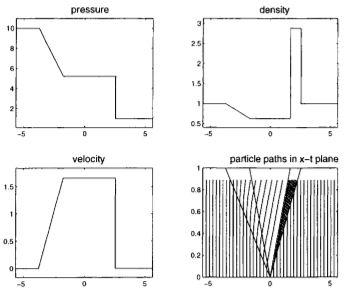
\includegraphics[width=1\linewidth]{Images/SODleveque}
%	\caption{Επίλυση του προβλήματος Riemann για τις μονοδιάστατες εξισώσεις Euler με αρχικές συνθήκες όπου η αρχική πίεση στα αριστερά είναι 10πλάσια της αρχικής πίεσης στα δεξιά ενώ οι αρχικές πυκνότητες μένουν ίδιες. Οι χαρακτηριστικές ταχύτητες είναι διαφορετικές (τελευταίο σχήμα) με αποτέλεσμα τα σωματίδια να πυκνώνουν και να δημιουργούν ένα κρουστικό κύμα πύκνωσης προς τα δεξιά, ενώ προς τα αριστερά δημιουργείται ένα κύμα αραίωσης. \cite{leveque_computational_1998}}
%\end{marginfigure}



\subsection{Αριθμητική επίλυση υπερβολικών εξισώσεων}
Η αριθμητική επίλυση των υπερβολικών εξίσωσεων αποτελεί μια δύσκολη διαδικασία
\subsubsection{Μέθοδος πεπερασμένων διαφορών}
Η βασική αρχή της μεθόδου των πεπερασμένων διαφορών -όπως και μεθόδων που πηγάζουν από αυτή και θα δούμε στη συνέχεια- είναι η διακριτοποιήση του χώρου και του χρόνου. Δηλαδή αναζητούμε μια προσεγγιστική τιμή των προς αναζήτηση ποσοτήτων σε συγκεκριμένα σημεία στο χώρο και στο χρόνο. Αν διακριτοποιήσουμε το χώρο κατα αποστάσεις $\Delta x=\Delta y = h$ και στο χρόνο $\Delta t=k$ τότε η προσεγγιστική τιμή στη θέση $(x_\mathrm{i},y_\mathrm{j})=(x_0+\mathrm{i}h,y_0+\mathrm{j}h)$ και στο χρόνο $t_\mathrm{n}=t_0+\mathrm{n}k$ θα είναι:
\begin{equation}
Q_{\mathrm{ij}}^\mathrm{n }\simeq q(x_\mathrm{i},y_\mathrm{j},t_\mathrm{n})
\end{equation}
Οπότε μια (για παράδειγμα μονοδιάτατη) μερική διαφορική εξίσωση της μορφής
\begin{equation}
\pdv{q}{t}+u\pdv{q}{x}=0
\end{equation} 
θα γράφεται:
\begin{equation}
\frac{Q_\mathrm{i}^\mathrm{n+1}-Q_\mathrm{i}^n }{k} + u \left( \frac{Q_\mathrm{i}^\mathrm{n+1}-Q_\mathrm{i}^\mathrm{n} }{k}  \right) =0
\end{equation}
άρα με βάση τις αρχικές συνθήκες $q_i^0$ μπορούμε να ολοκληρώσουμε στο χρόνο, άρα η λύση στο κελί με συντεταγμένες $\mathrm{ijn}$ θα είναι:
\begin{equation}
Q_{\mathrm{i}}^\mathrm{n+1} = Q_{\mathrm{i}}^\mathrm{n} -\frac{k}{h} u \left( Q_\mathrm{i}^\mathrm{n} - Q_\mathrm{i-1}^\mathrm{n} \right)
\end{equation} 

Αντίστοιχα στη περίπτωση ενός συστήματος εξισώσεων η λύση θα ήταν
\begin{equation}
Q_{\mathrm{i}}^\mathrm{n+1} = Q_{\mathrm{i}}^\mathrm{n} -\frac{k}{h} \mathbf{Α} \left( Q_\mathrm{i}^\mathrm{n} - Q_\mathrm{i-1}^\mathrm{n} \right)
\end{equation} 
με τον πίνακα $\mathbf{Α}$ να έχει θετικές ιδιοτιμές. 

Η τιμή των ποσοτήτων σε ένα κελί παρατηρούμε ότι εξαρτάται από τις τιμές των αμέσως γειτονικών κελιών. Η ακρίβεια μας τώρα είναι της τάξης του $h$ \todo{γιατί? Taylor}. Για να πετύχουμε μεγαλύτερη ακρίβεια μπορούμε να ανανεώνουμε τις ποσότητες $q_j$ με βάση πιο απομακρυσμένα κελιά, όπως για παράδειγμα η μέθοδος leapfrog:
\begin{equation}
Q_{\mathrm{i}}^\mathrm{n+1} = Q_{\mathrm{i}}^\mathrm{n-1} -\frac{k}{h} \mathbf{Α} \left( Q_\mathrm{i+1}^\mathrm{n} - Q_\mathrm{i-1}^\mathrm{n} \right)
\end{equation} 
ή να κρατήσουμε τους 3 πρώτους όρους από το αναπτύγμα Taylor $q(x,t+k)=q(x,t)+k\pdv{q}{t}(x,t)+\frac{1}{2}k^2 \pdv[2]{q}{t}$ τη μέθοδο Lax-Wendroff:
 
 \begin{equation}
 Q_{\mathrm{i}}^\mathrm{n+1} = Q_{\mathrm{i}}^\mathrm{n} -\frac{k}{2h} \mathbf{Α} \left( Q_\mathrm{i+1}^\mathrm{n} - Q_\mathrm{i-1}^\mathrm{n} \right) +\frac{k^2}{2h^2} \mathbf{Α}^2 \left( Q_\mathrm{i+1}^\mathrm{n} - 2Q_{\mathrm{i}}^\mathrm{n}+ Q_\mathrm{i-1}^\mathrm{n} \right)
 \end{equation} 
 
 Παρά το βαθμό ακρίβεια της κάθε μέθοδο μεταξύ των παραπάνω, οι μέθοδοι πεπερασμένων διαφορών δεν καταφέρνουν να διατηρήσουν τις ολοκληρώσιμες ποσότητες ειδικά όταν εμπλέκονται κρουστικά κύματα και ασυνέχειες. Γι αυτό το σκοπό θα χρησιμοποιήσουμε τις λεγόμενες μεθόδους πεπερασμένων όγκων.
 
\subsubsection{Μέθοδος Πεπερασμένων Όγκων}
Αντί για τη προσεγγιστική τιμή $Q_{\mathrm{i}}^\mathrm{n+1}$ της $q(x_\mathrm{i},t_\mathrm{n+1})$ σε ένα συγκεκριμένο σημείο θα ορίσουμε μια νέα αντίστοιχη τιμή για τη μέση τιμή της ποσότητας σε κάθε ένα διάστημα $C_\mathrm{i}=[x_\mathrm{i},x_\mathrm{i+1}]$ του χώρου μας με $x_\mathrm{i}=x_0+(i-1)h$. 

Άρα τώρα η τιμή $Q_{\mathrm{i}}^\mathrm{n}$ θα προσεγγίζει την μέση τιμή στο $\mathrm{i}$ διάστημα τη χρονική στιγμή $t_\mathrm{n}$
\begin{equation}
Q_{\mathrm{i}}^\mathrm{n} \simeq \frac{1}{h} \int _{C_\mathrm{i}} q(x,t_\mathrm{n})dx
\end{equation}
Αν η $q(x,t)$ δεν περιέχει ασυνέχειες τότε η $Q_{\mathrm{i}}^\mathrm{n}$ τη προσεγγίζει στο μέσο του διαστήματος με ακρίβεια τάξης μεγέθους $\order{h^2}$.

Αν πάρουμε την ολοκληρωτική μορφή του νόμου διατήρησης σε ένα κελί η εξέλιξη στο χρόνο θα είναι
\begin{equation}
\int _{C_\mathrm{i}} q(x,t_\mathrm{n+1})dx -\int _{C_\mathrm{i}} q(x,t_\mathrm{n})dx = 
\int_{t_\mathrm{n}}^{t_\mathrm{n+1}} f(q(x_\mathrm{i},t))dt - \int_{t_\mathrm{n}}^{t_\mathrm{n+1}} f(q(x_\mathrm{i+1},t))dt
\end{equation}

\marginpar{
Αν αναδιατάξουμε τη σχέση \ref{eq:FVM} κατάλληλα βρίσκουμε:
\begin{equation}
\frac{Q_{\mathrm{i}}^\mathrm{n+1} - Q_{\mathrm{i}}^\mathrm{n}}{k} +\frac{F_{\mathrm{i+1}}^\mathrm{n} - F_{\mathrm{i}}^\mathrm{n}}{h}=0
\end{equation}
η οποία είναι η εξίσωση του νόμου διατήρησης. Ακρι
}
\begin{marginfigure}
	\centering
	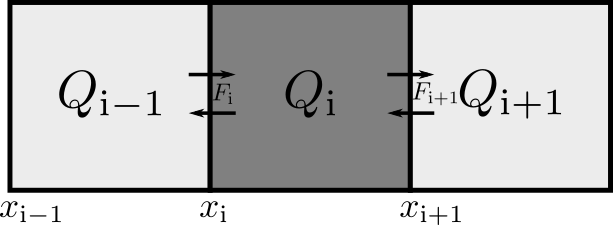
\includegraphics[width=1\linewidth]{Images/FVM}
	\caption{}
	\label{fig:fvm}
\end{marginfigure}


διαιρώντας με $h$ και αντικαθιστώντας τις $Q_{\mathrm{i}}^\mathrm{n}$ βρίσκουμε την εξέλιξη στο χρόνο
\begin{equation}
Q_{\mathrm{i}}^\mathrm{n+1} = Q_{\mathrm{i}}^\mathrm{n} - \frac{1}{h}\left( \int_{t_\mathrm{n}}^{t_\mathrm{n+1}} f(q(x_\mathrm{i},t))dt - \int_{t_\mathrm{n}}^{t_\mathrm{n+1}} f(q(x_\mathrm{i+1},t))dt \right) 
\end{equation}
και τελικά
\begin{equation}
\label{eq:FVM}
Q_{\mathrm{i}}^\mathrm{n+1} = Q_{\mathrm{i}}^\mathrm{n} - \frac{k}{h}\left(F_{\mathrm{i+1}}^\mathrm{n}-F_{\mathrm{i}}^\mathrm{n} \right) 
\end{equation}
όπου 
\begin{equation}
F_{\mathrm{i}}^\mathrm{n} \simeq \frac{1}{k}\int_{t_\mathrm{n}}^{t_\mathrm{n}}f(q(x_\mathrm{i},t))dt 
\end{equation}
η προσεγγιστική τιμή της μέσης ροής κατά μήκος της $x_\mathrm{i}$. Είναι λογικό να υποθέσουμε ότι η ροή στο σύνορο μεταξύ δύο κελιών εξαρτάται από τις τιμές των ποσοτήτων σε αυτά τα δύο κελιά, δηλαδή %η συνάρτηση της ροής
\begin{equation}
F_{\mathrm{i}}^\mathrm{n} = F\left( Q_{\mathrm{i-1}}^\mathrm{n} ,Q_{\mathrm{i}}^\mathrm{n} \right) 
\end{equation}
άρα αν γνωρίζουμε αυτή τη συνάρτηση ροής τότε μπορούμε να υπολογίσουμε την εξέλιξη στο χρόνο της μέσης τιμής του κάθε κελιού
\begin{equation}
Q_{\mathrm{i}}^\mathrm{n+1} = Q_{\mathrm{i}}^\mathrm{n} - \frac{k}{h}\left(
F\left( Q_{\mathrm{i}}^\mathrm{n} ,Q_{\mathrm{i+1}}^\mathrm{n} \right)-
F\left( Q_{\mathrm{i-1}}^\mathrm{n} ,Q_{\mathrm{i}}^\mathrm{n} \right)
 \right) 
\end{equation} 

Η μέθοδος (ή καλύτερα η οικογένεια μεθόδων) που ακολουθούμε στην εύρεση των συναρτήσεων ροής ονομάζεται μέθοδος Godunov, από τον Sergei K. Godunov που πρώτος την εισήγαγε το 1959. Η μέθοδος αυτή βασίζεται στην επίλυση του προβλήματος Riemann μεταξύ των κελιών.
Παρακάτω θα αναπτύξουμε το πως λύνεται το πρόβλημα Riemann.
 

\subsection{Πρόβλημα Riemann}
Το πρόβλημα Riemann είναι η επίλυση του νόμου διατήρησης της μορφής
\begin{equation}
\pdv{\bar{q}}{t}+\pdv{f(\bar{q})}{x}=0
\end{equation}
με αρχικές συνθήκες όπου υπάρχει μια ασυνέχεια:
\begin{equation}
\bar{q}(x,0)=
\begin{cases}
\bar{q}_\mathrm{L} &\qq{για} x<0 \\
\bar{q}_\mathrm{R} &\qq{για} x>0 
\end{cases}
\end{equation}

%Όπως βλέπουμε χαρακτηριστικά και στο shock tube problem (\ref{fig:sodleveque}), λόγω της αρχικής ασυνέχειας και της μη-γραμμικότητας των εξισώσεων euler έχουμε σαν αποτέλεσμα τη δημιουργία κρουστικών κυμάτων.
Για να δώσουμε μια αναλυτική λύση στο γενικό πρόβλημα (μη-γραμμικό) Riemann θα ξεκινήσουμε από τη γραμμική περίπτωση.

\subsubsection{Γενική επίλυση του γραμμικού προβλήματος Riemann}
Η επίλυση του προβλήματος Riemann στη γραμμική περίπτωση του νόμου διατήρησης, δηλαδή στο σύστημα
\begin{equation}
\pdv{\bar{q}}{t} +  \mathbf{A}\pdv{\bar{q}}{x}  = 0 
\end{equation}
 βασίζεται στο μετασχηματισμό των ποσοτήτων $\bar{q}$ στις λεγόμενες χαρακτηριστικές μεταβλητές $\bar{\xi}=\mathbf{R}^{-1}\bar{q}$ όπου $\mathbf{R}=(\bar{r}_1,\bar{r}_2,\cdots \bar{r}_m)$ είναι ο πίνακας των ιδιοανυσμάτων του πίνακα $\mathbf{A}$, ενώ με $\bar{\Lambda}=\mathtt{diag}(\lambda _1,\lambda _2,\cdots \lambda _m)$ ορίζουμε το διαγώνιο πίνακα των ιδιοτιμών. Για τον πίνακα $\mathbf{A}$ ισχύει\ ότι $\mathbf{A}=\mathbf{R}\bar{\Lambda}\mathbf{R}^{-1}$.

Οι εξισώσεις τότε γράφονται:
\begin{equation}
\pdv{\bar{\xi}}{t} + \bar{\Lambda} \div\bar{\xi} =0
\end{equation} 
δηλαδή σαν ένα διαχωρισμένο σύστημα εξισώσεων της μορφής 
\begin{equation}
\pdv{q}{t} +  u\pdv{q}{x}  = 0 
\end{equation} που όπως έχουμε δει ήδη έχουν λύσεις:
\begin{equation}
\label{eq:xi_solution}
\xi_p  = \xi_p(x-\lambda _p t,0) 
\end{equation}
με $p=1...m$ για τις $m$ εξισώσεις (μονοδιάστατη περίπτωση). Οι $p$ χαρακτηριστικές καμπύλες δηλαδή καθορίζονται από τις ιδιοτιμές $\lambda _p$.

Άρα αν επιστρέψουμε στις αρχικές μεταβλητές:
\begin{equation}
\bar{q}(x,t) = \sum_{p=1}^{m} \xi_p(x-\lambda _p t,0)\bar{r}_p
\end{equation}

\begin{marginfigure}
	\centering
	\label{fig:linearriemann-leveque}
	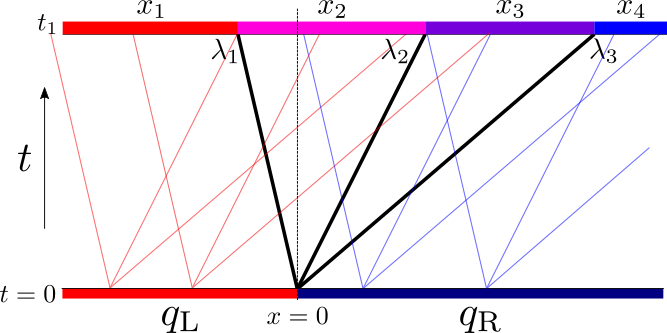
\includegraphics[width=1\linewidth]{Images/reimannlinear.png}
	\caption{Γραφική απεικόνιση της λύση του γραμμικού προβλήματος Riemann για $p=3$. 
		Τη χρονική στιγμή $t_1$ οι λύσεις σε κάθε σημείο του χώρου καθορίζονται απόλυτα από τις $p$ χαρακτηριστικές ιδιοτιμές $\lambda _p$ έτσι ώστε η τελική λύση για κάθε σημείο $x$ να είναι ο γραμμικός συνδυασμός των περιοχών που επηρεάζουν αυτό το σημείο, δηλαδή}	
	\begin{align*}
	q(x_1,t_1)&=\xi _1 ^L r_1 +\xi _2 ^L r_2 + \xi _3 ^L r_3 \\
	q(x_2,t_1)&=\xi _1 ^R r_1 +\xi _2 ^L r_2 + \xi _3 ^L r_3 \\
	q(x_3,t_1)&=\xi _1 ^R r_1 +\xi _2 ^R r_2 + \xi _3 ^L r_3 \\
	q(x_4,t_1)&=\xi _1 ^R r_1 +\xi _2 ^R r_2 + \xi _3 ^R r_3 
	\end{align*} 
	
\end{marginfigure}
Για τις αρχικές συνθήκες του προβλήματος Riemann o μετασχηματισμός μας δίνει:
\begin{equation}
\xi_p (x,0) =
\begin{cases}
\xi^\mathrm{L}_p &\qq{για} x<0 \\
\xi^\mathrm{R}_p &\qq{για} x>0 
\end{cases}
\end{equation} 

άρα από \ref{eq:xi_solution}
\begin{equation}
\xi_p (x,t) =
\begin{cases}
\xi^\mathrm{L}_p &\qq{για} x-\lambda _p t<0 \\
\xi^\mathrm{R}_p &\qq{για} x-\lambda _p t>0 
\end{cases}
\end{equation} 




Άρα με αρχικές συνθήκες Riemann, βλέπουμε ότι η λύση για τις μετασχηματισμένη μεταβλητή $\xi _p$ σε ένα οποιαδήποτε σημείο εξαρτάται απόλυτα αό τη σχετική θέση σε σχέση με την αντίστοιχη χαρακτηριστική καμπύλη της $\lambda _p$.  

Καθώς διασχίζουμε τη καμπύλη αυτή ουσιαστικά μετακινούμαστε από τις συνθήκες $\xi^L_p$ στις $\xi^R_p$. Το άλμα αυτό υπακούει τις συνθήκες Rankine-Hugoniot \todo{Rankine-Hugoniot} άρα για κάθε σημείο μπορούμε τελικά να γράψουμε τη λύση.
\begin{equation}
\bar{q}(x,t)=q_L + \sum_{\lambda_p<x/t} (\xi ^R_P - \xi ^L_P) \bar{r_p}
			=q_R - \sum_{\lambda_p>x/t} (\xi ^R_P - \xi ^L_P) \bar{r_p}
\end{equation}
\todo{Επιλυση γραμμικου Riemann διαγραμμα}

\subsubsection{Επίλυση του μη γραμμικού προβλήματος Riemann}
Στη μη γραμμική περίπτωσή των νόμων διατήρησης, όπως είναι και οι εξισώσεις Euler, η συνάρτηση ροής της διατηρούμενης ποσότητας εξαρτάται πια από την ίδια τη ποσότητα, δηλαδή:
\begin{equation}
\pdv{t} \bar{q}(x,t) + \pdv{x} \bar{f}(\bar{q}(x,t)) = 0 
\end{equation}

Για ομαλές λύσεις μπορούμε να μετασχηματίσουμε το παραπάνω σύστημα μέσω της ιακωβιανής $\mathbf{J} =\mathbf{f}'$
\begin{equation}
\pdv{t} \bar{q}(x,t) + \mathbf{J}(q(x,t)) \pdv{q}{x}  = 0 
\end{equation}

Λειτουργώντας όπως και στη γραμμική περίπτωση παρατηρούμε ότι οι ιδιοτιμές και τα ιδιοανύσματα της ιακωβιανής είναι συναρτήσεις των ποσοτήτων $q_\mathrm{j}$. Δηλαδή οι κλίσεις των χαρακτηριστικών καμπύλων μπορούν να αλλάζουν στο χώρο και στο χρόνο. 

\begin{marginfigure}
	\centering
	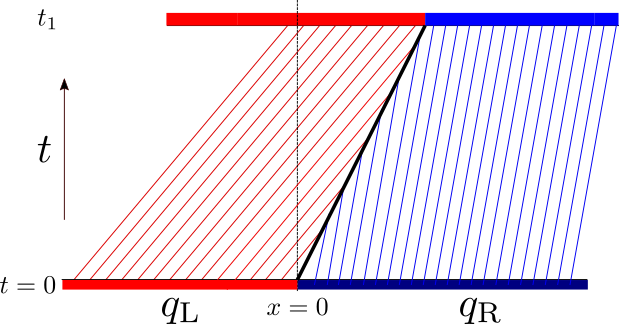
\includegraphics[width=1\linewidth]{Images/shockwave}
	\caption{}
	\label{fig:shockwave}
\end{marginfigure}


\begin{marginfigure}
	\centering
	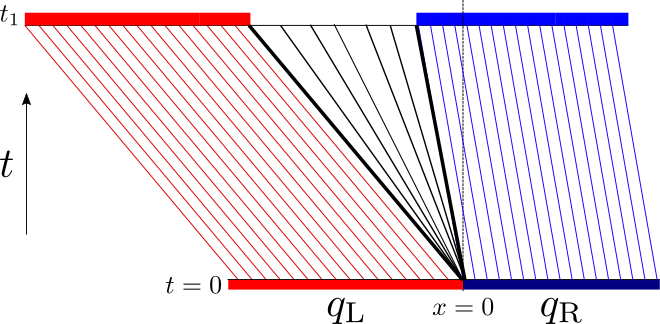
\includegraphics[width=1\linewidth]{Images/rarefuctionwave}
	\caption{}
	\label{fig:rarefuctionwave}
\end{marginfigure}

Συμπεραίνουμε λοιπόν ότι σε περιοχές ανάμεσα σε αυτές οι λύσεις περιγράφονται ακριβώς όπως και στη γραμμική περίπτωση, ενώ ταυτόχρονα έχουμε και τη δημιουργία 2 νέων "χαρακτηριστικών" καμπυλών - κυμάτων στα σημεία μεταξύ αυτών των περιοχών.

Στις περιοχές όπου οι χαρακτηριστικές καμπύλες συγκλίνουν έχουμε τα λεγόμενα κρουστικά κύματα τα οποία διαδίδονται με ταχύτητα \todo{shock wave speed} και στις περιοχές που αποκλίνουν τα κύματα αραίωσης.

Άρα για να υπολογίσουμε 
\todo{Ολοκλήρωσε το}




\subsection{Κώδικας PLUTO}


	\section{Ορισμός του test problem}
	Πριν προχωρήσουμε σε πολύπλοκες διαδικασίες, θα πρέπει να εξετάσουμε την απόδοση και την ευστάθεια του κώδικα PLUTO σε κάποια περισσότερο "απλοικά" σενάρια. Γι αυτό το λόγο θα ορίσουμε ένα test problem με ένα σφαιρικό, ομοιογενές νέφος που βρίσκεται αρχικά σε ισορροπία πίεσης με το διαγαλαξιακό χώρο. 
	
	\subsection{Αρχικές Συνθήκες}
	\label{par:InitialConditions}
	Θεωρούμε ένα στατικό μοριακό νέφος ακτίνας $\SI{10} {pc}$ με αριθμητική πυκνότητα
	της τάξης των $\SI{1000}{cm^{-3}}$ δηλαδή πυκνότητας $\rho=\SI{1.67e-21}{g. \cm^{-3}}$ και θερμοκρασίας $T=\SI{100}{\kelvin}$.
	Για το διαγαλαξιακό μέσο θεωρούμε αντίστοιχα μια αριθμητική πυκνότητα της τάξης του 
	$\SI{1}{\cm^{-3}}$ δηλαδή $\rho=\SI{1.67e-24}{g. \cm^{-3}}$ και θερμοκρασία $T=\SI{1e5}{\kelvin}$.

			\begin{marginfigure}
				\centering
				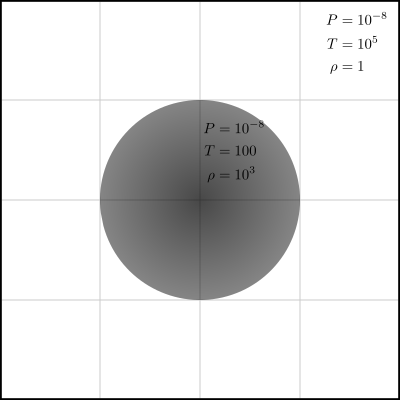
\includegraphics[width=0.7\linewidth]{Images/rect4578.png}
				\caption{Αρχικές συνθήκες ενός στατικού σφαιρικού νέφους ακτίνας \SI{10}{pc}}
				\label{fig:rect4578}
			\end{marginfigure}
		

	
	\subsection{Μονάδες κώδικα}
	Για τις ολοκληρώσεις ο PLUTO χρησιμοποιεί αδιάστατες μεταβλητές για τις ποσότητες πίεσης, πυκνότητας, ταχύτητας, χρόνου και θέσης έτσι ώστε οι αριθμητικές τιμές να εμπίπτουν σε πλαίσια που αποφεύγονται αριθμητικά σφάλματα ($>\num{1e-9},<\num{1e12}$). Στο παρακάτω πίνακα ορίζουμε τις νέες μονάδες, τις οποίες ονομάζουμε και μονάδες κώδικα: 
	
			\begin{table}[H]
				\centering
				\caption{Code Units}
				\label{tab:cd}
				\begin{tabular}{|l|  c |  l|}
					\toprule
					Quantity & Symbol & Code Unit\\ 
					\midrule
					Length & $L_0$ & $\SI{3e19}{\cm} = \SI{10}{pc}$ \\
					Velocity & $V_0$ & $\SI{3e10}{\cm \sec^{-1}}$\\
					Density& $\rho_0$&$\SI{1.67e-24}{g.\cm^3}$\\
					%\multirow{2}{*}{Mass \\ Density} &\multirow{2}{*}{$\rho_0$}  & \multirow{2}{*}{$\SI{1.67e-21}{g. \cm^{-3}}$} \\ \\
					Time & $t_0=\frac{L_0}{V_0}$ & $10^9\si{\sec} =\SI{32}{yrs}$\\
					Pressure & $P_0=\rho_0 V_0^2$ &$\SI{1.5e-3}{dyn.cm^{-2}}$ \\
					Temperature &$T_0=\frac{V_0^2m_p}{k_b}$&$10^{13}\si{\kelvin}$  \\		
					\bottomrule
				\end{tabular}
			\end{table}

	\todo{Βάλε τι ρυθ7μίσεις κάναμε στο PLUTO από τα pluto.ini}
	
	\section{Σφαιρικό νέφος μέσα στην ISM}

	Αρχικά θα εκτελέσουμε τη προσομοίωση μας χωρίς καμία "ιδιαίτερη" φυσική διεργασία, δηλαδή θα αφήσουμε ελεύθερο ένα πυκνό σφαιρικό νέφος με τις παραπάνω αρχικές συνθήκες μέσα στο αραιό-θερμό διαγαλαξιακό αέριο.
	
 Όπως παρατηρούμε από το σχήμα~\ref{fig:NoCoolingRHOquad} και καλύτερα από το σχήμα~\ref{fig:nocoolingrhoprofile} μέσα σε 8 εκατομμύρια χρόνια το νέφος είναι στη πράξη σταθερό. 
 
 \begin{marginfigure}
 	\centering
 	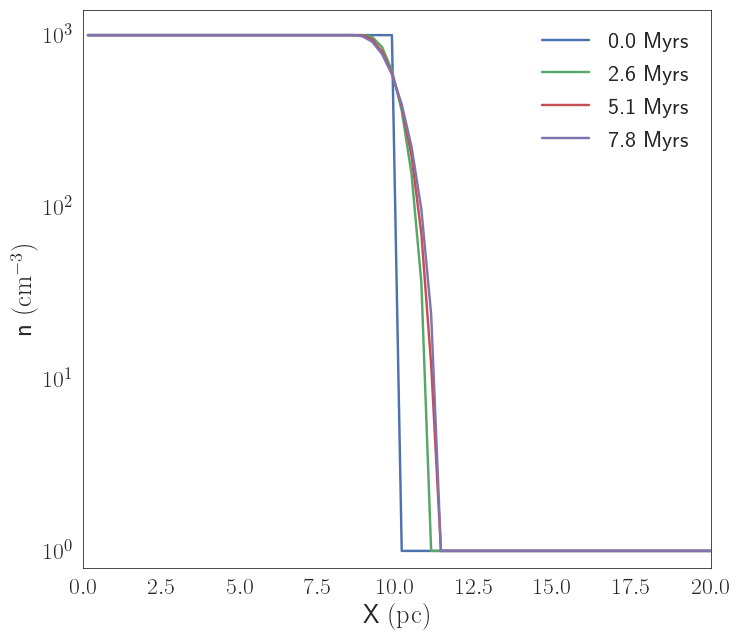
\includegraphics[width=1.0\linewidth]{DataImages/NoCoolingRHOprofile}
 	\caption{Προφίλ της πυκνότητας κατά μήκος της ευθείας $y=0$.}
 	\label{fig:nocoolingrhoprofile}
 \end{marginfigure}	
 
  Η φαινομενική διάχυση που παρατηρούμε είναι αποτέλεσμα αριθμητικών σφαλμάτων στις ταχύτητες (τάξης των \num{1e-18}) καθώς δεν παίρνουμε υπ όψιν μας τη μοριακή διάχυση. Η διάχυση προσθέτει έναν ελλειπτικό όρο στις εξισώσεις με συνέπεια μεγαλύτερη αριθμητική αστάθεια. Καθώς η διάχυση αφορά πολύ μικρές χωρικές κλίμακες τη θεωρούμε αμελητέα \todo{δειξε το αυτό} 
  Η πίεση παραμένει παντού σταθερή και γι αυτό το σχετικό διάγραμμα παραλείπεται.  
 	
	\begin{figure}[h]
		\centering
		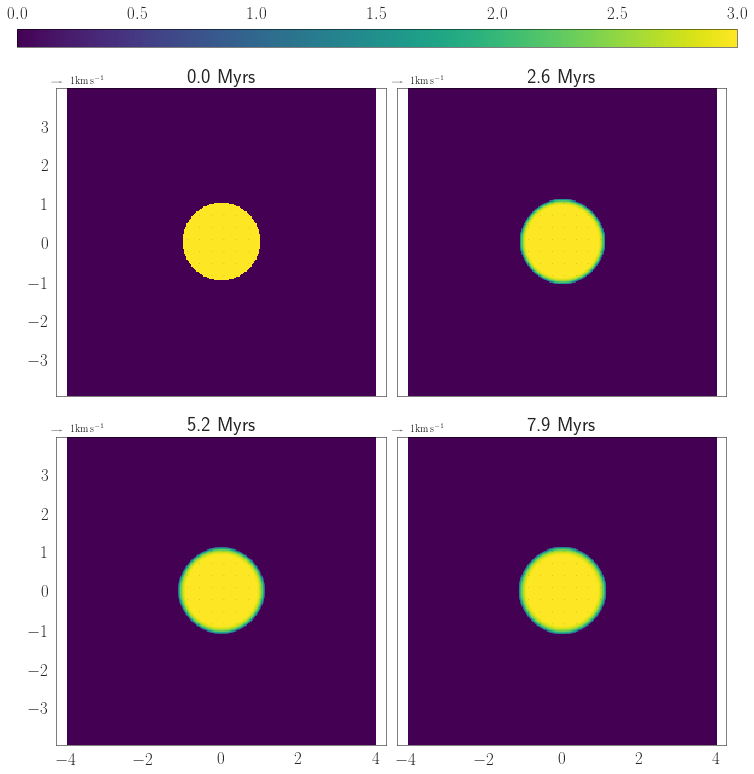
\includegraphics[width=1.0\linewidth]{DataImages/NoCoolingRHOquad}
		\label{fig:NoCoolingRHOquad}
		\caption{Στιγμιότυπα της πυκνότητας ενός σφαιρικού νέφους έως τα 8 εκατομμύρια χρόνια.}
	\end{figure}	
	
	\section{Σφαιρικό νέφος με Radiation Cooling}
	Σκοπός μας είναι να εστιάσουμε στην επιρροή της ψύξης στη δυναμική του αερίου. Ο PLUTO μας δίνει αυτή τη δυνατότητα με τη χρήση διάφορων modules όπου το αέριο ψύχεται καθώς ακτινοβολεί (Radiation Cooling). 

	\subsection{Οπτικό βάθος}
	Το νέφος έχει αριθμητική πυκνότητα $\SI{1000}{atoms.cm^{-3}}$ άρα το οπτικό βάθος για ένα φωτόνιο που εκπέμπεται μέσα στο νέφος είναι:
	\begin{equation}
	\tau = nL\sigma _T\simeq \num{6.65e-3}
	\end{equation}
	όπου $\sigma _T = \SI{6.65e-25}{cm^2}$ είναι η ενεργός διατομή Thomson.
	
	Έτσι μπορούμε να συμπεράνουμε οτι είναι οπτικά αδιαφανές, άρα θεωρούμε ότι η ψύξη θα γίνεται ταυτόχρονα σε όλο τον όγκο του νέφους. 
	
	\subsection{Tabulated Cooling}
	Το πρώτο cooling module που θα χρησιμοποιήσουμε ονομάζεται Tabulated Cooling, το οποίο υπολογίζει τον όρο ψύξης $\Lambda (T )$ στην εξίσωση ενέργειας 
	\begin{equation}
		\pdv{t}(\rho e)=-\Lambda^*(n,T)=-n^2 \Lambda(T)
	\end{equation}
	
		\begin{marginfigure}
		%\centering
		\caption{Παράμετρος ψύξης $\Lambda$}
		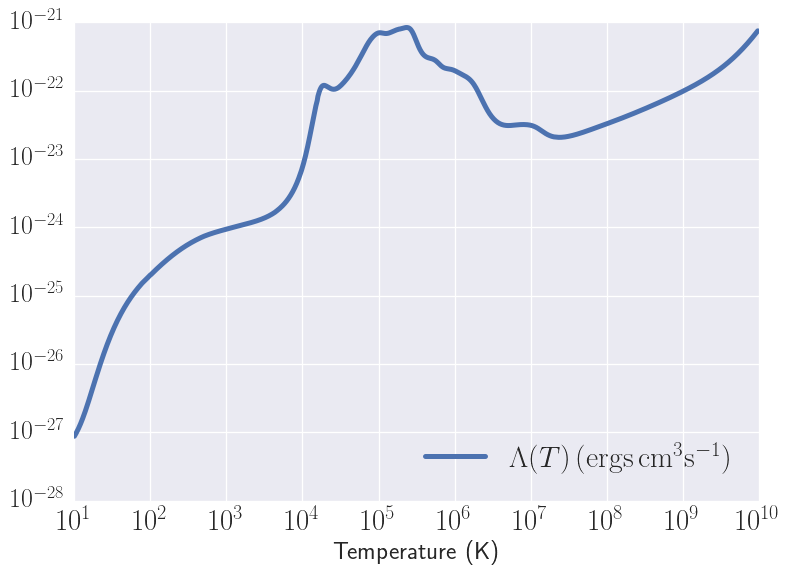
\includegraphics[width=1.0\linewidth]{Images/LambdaT}
		\label{fig:LambdaT}
	\end{marginfigure}
 με αριθμητικές τιμές από έναν εμπειρικό πίνακα καθώς δεν έχουμε αναλυτική μορφή τη συνάρτησης ψύξης. 
 Η μορφή της $\Lambda(T)$ εξαρτάται από τη μεταλλικότητα του αερίου, καθώς οι γραμμές εκπομπής (για θερμοκρασίες \SIrange{1e4}{1e7}{K}) των μετάλλων κυριαρχούν. Για θερμοκρασίες ανώτερες των \SI{1e7}{K} κυριαρχεί η ακτινοβολία bremmstrahlung ενώ για χαμηλότερες των \SI{1e4}{K} η ψύξη προέρχεται από μοριακές εκπομπές (\ce{H2},\ce{CO} κλπ). 
 
 Οι εμπειρικές τιμές της $\Lambda(T)$ που χρησιμοποιήσαμε έχουν παραχθεί από το λογισμικό cloudy με αναλογίες αντίστοιχες της ηλιακής ατμόσφαιρας φαίνονται στο σχήμα~\ref{fig:LambdaT}) σε μονάδες $ \si{ergs.\cm^3 s^{-1}}$ και για  $n=\frac{\rho}{\mu m_u}$.

Η "απλότητα" του συγκεκριμένου module το οποίο δεν συμπεριλαμβάνει τις χημικές διεργασίες, όπως θα δούμε παρακάτω, του προσδίδει αφενός το πλεονέκτημα των χαμηλών υπολογιστικών απαιτήσεων αλλά και την ευκολία στο να κάνουμε μια πρώτη εκτίμηση της χρονικής εξέλιξης των φαινομένων.      
	
	\subsubsection{Χρονική κλίμακα ψύξης}
	Για μια αρχική θερμοκρασία $T=\SI{100}{K}$ και αριθμητική πυκνότητα $n=10^3\si{protons.cm^{-3}}$ από την εξίσωση της ενέργειας μπορούμε να εκτιμήσουμε τη χρονική κλίμακα ψύξης του νέφους:
	\marginpar{\centering $k_b=\SI{1.38e-16}{ergs.K^{-1}}$}
	\begin{equation}
		\tau _c =\frac{ \rho e} {n^2 \Lambda (T)}=
		\frac{ \frac{3}{2}k_b T} {n \Lambda (T)} 
		\simeq 10^8\si{s}\simeq \SI{3}{yrs}
	\end{equation}
	Βλέπουμε ότι η χρονική κλίμακα ψύξης είναι τάξης ετών, δηλαδή εξαιρετικά μικρή σε σχέση με τους χρόνους που προσομοιώνουμε (τάξης $10^5\si{yrs}$) και τους χρόνους δυναμικής των νεφών γενικά.
	
	Αν υπολογίσουμε την αντίστοιχη χρονική κλίμακα και για το εξωτερικό του νέφους βρίσκουμε περίπου \SI{600}{yrs}. 
	\todo{θα επρεπε το εξωτερικο να μένει σταθερα στους 10000?}

	\begin{marginfigure}
	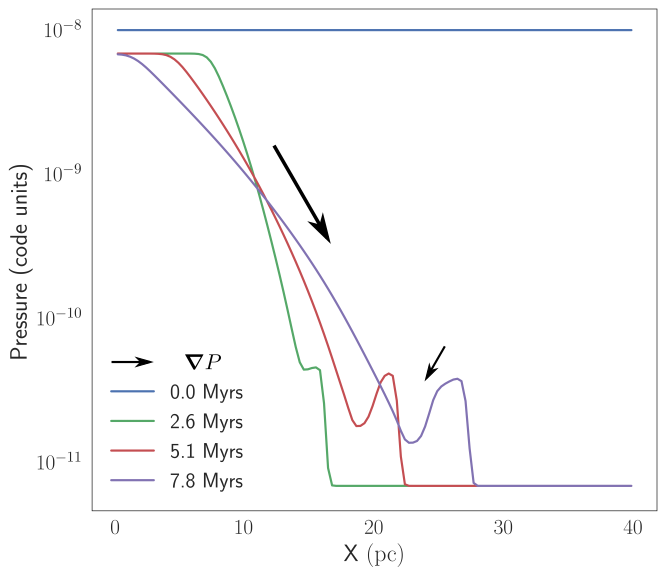
\includegraphics[width=1\linewidth]{DataImages/TabCoolingPRSprofile-gradP}
	\caption{Το προφίλ της πίεσης του αερίου με ενεργοποιημένο το Tabulated Cooling Module κατά μήκος της ευθείας $y=0$ με το χρόνο. Ενδεικτικά (εκτός κλίμακας) δείχνουμε και τη κλίση της πίεσης.}
	\label{fig:tabcoolingprsprofile-gradp}
\end{marginfigure}

\begin{marginfigure}
	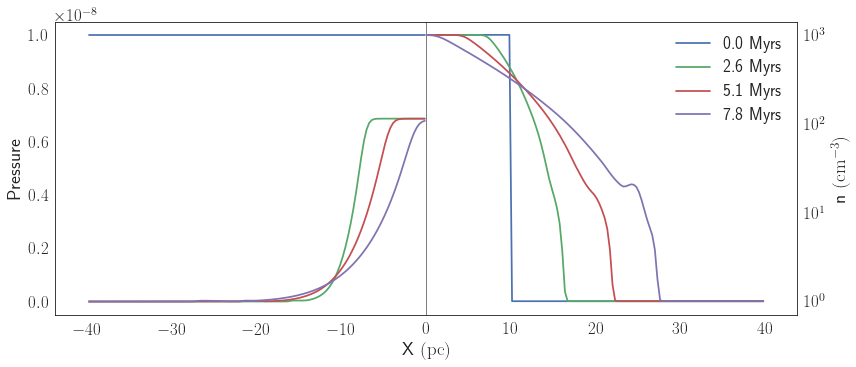
\includegraphics[width=1\linewidth]{DataImages/TabCoolingRHOprofile}
	\caption{Το προφίλ της πυκνότητας του αερίου με ενεργοποιημένο το Tabulated Cooling Module κατά μήκος της ευθείας $y=0$ με το χρόνο.} 
	\label{fig:tabcoolingrhoprofile}
\end{marginfigure}	

	\subsubsection{Δυναμική του νέφους}
	
	Το αέριο στο εσωτερικό του νέφους κρυώνει γρηγορότερα απ' ότι στο εξωτερικό περιβάλλον με συνέπεια η πίεση $P \sim \rho T$ να μικραίνει γρηγορότερα στο εσωτερικό (εφόσον αρχικά είναι ίδια παντού). Αυτή η διαφορά πίεσης δημιουργεί μια  δύναμη η οποία θα έπρεπε να επιταχύνει το αέριο προς το εσωτερικό του. 
	
	\begin{figure}[h]
		\centering
		\caption{Ο χάρτης της πυκνότητας του νέφους στο χρόνο σε λογαριθμική κλίμακα.}
		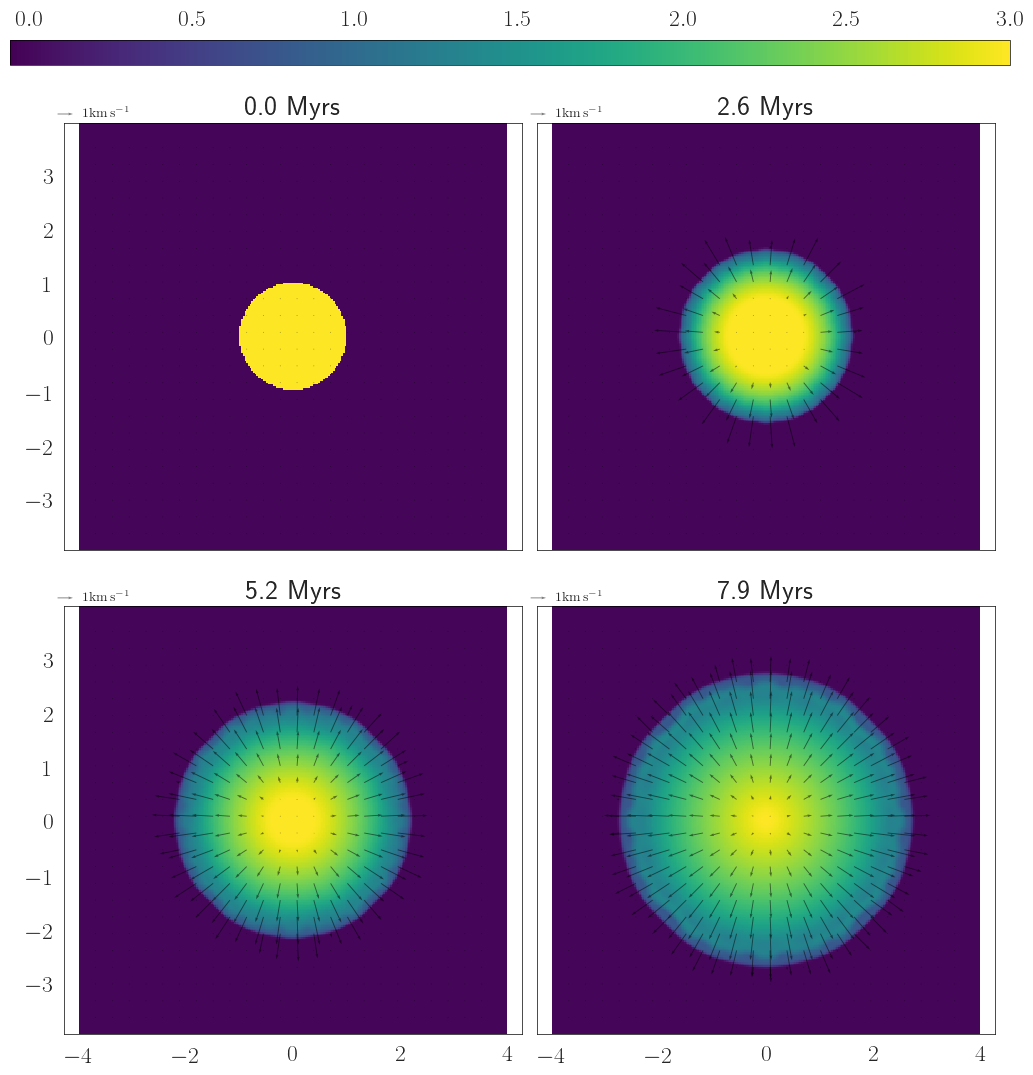
\includegraphics[width=1.0\linewidth]{DataImages/TabCoolingRHOquad}
		\label{fig:TabCoolingRHOquad}
	\end{figure}
	
	Από τις προσομοιώσεις όμως, βλέπε σχήματα (\ref{fig:tabcoolingprsprofile-gradp},\ref{fig:tabcoolingprsprofile-gradp}) παρατηρούμε το αντίθετο αποτέλεσμα, δηλαδή μια διαφορά πίεσης με φορά δύναμης προς τα έξω. 


%	\begin{figure}[h]
%		\begin{adjustwidth*}{-5cm}{-0cm}%
%		\centering
%		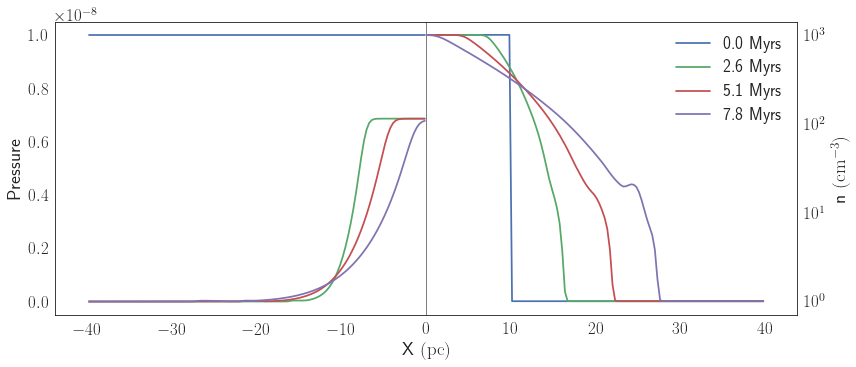
\includegraphics[width=1\linewidth]{DataImages/TabCoolingRHOprofile}
%		\caption{Το προφίλ της πυκνότητας του αερίου με ενεργοποιημένο το Tabulated Cooling Module κατά μήκος της ευθείας $y=0$ με το χρόνο.}
%		\label{fig:tabcoolingrhoprofile}
%		
%		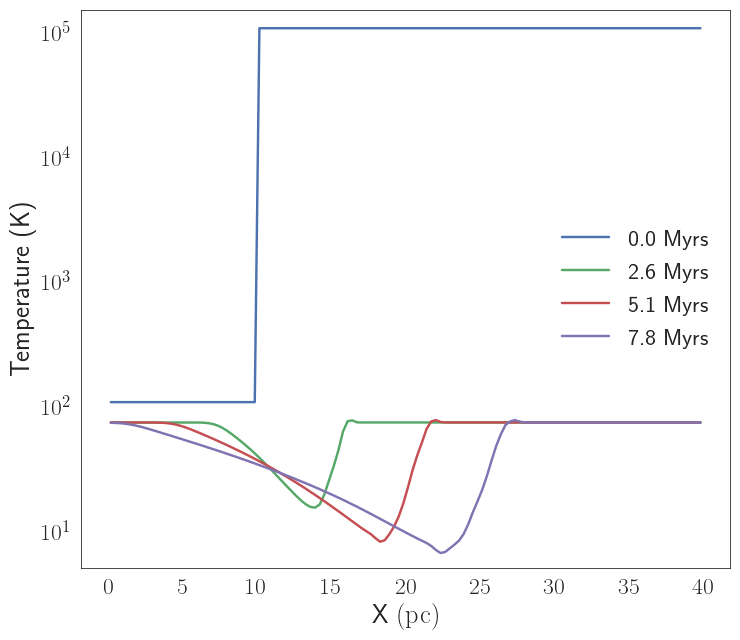
\includegraphics[width=1\linewidth]{DataImages/TabCoolingTMPprofile}
%		\caption{Το προφίλ της θερμοκρασίας του αερίου με ενεργοποιημένο το Tabulated Cooling Module κατά μήκος της ευθείας $y=0$ με το χρόνο.}
%		\label{fig:tabcoolingtmpprofile}
%		
%		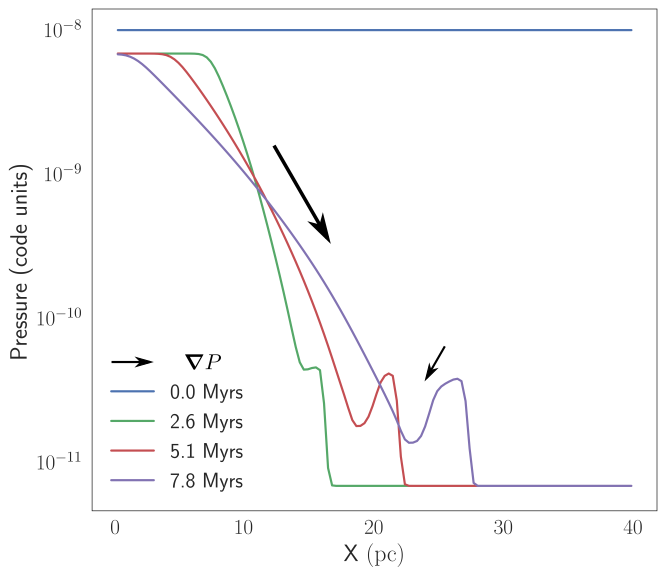
\includegraphics[width=1\linewidth]{DataImages/TabCoolingPRSprofile-gradP}
%		\caption{Το προφίλ της πίεσης του αερίου με ενεργοποιημένο το Tabulated Cooling Module κατά μήκος της ευθείας $y=0$ με το χρόνο. Ενδεικτικά (εκτός κλίμακας) δείχνουμε και τη κλίση της πίεσης.}
%		\label{fig:tabcoolingprsprofile-gradp}
%	\end{adjustwidth*}
%	\end{figure}

	
\begin{marginfigure}
	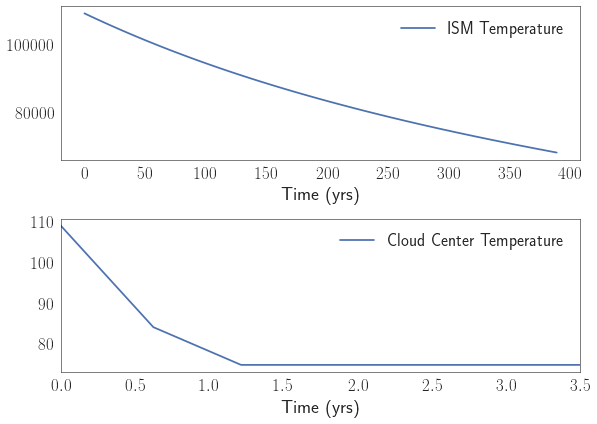
\includegraphics[width=1\linewidth]{DataImages/TabCoolingTMPcenterISM}
	\caption{Η θερμοκρασία στο κέντρο του νέφους συναρτήσει του χρόνου σε ακρίβεια τάξης ετών}
	\label{fig:tabcoolingtmpcenter}
\end{marginfigure}
	
	Για να μελετήσουμε αυτή τη "παράδοξη" συμπεριφορά διαφορά επαναλάβαμε την προσομοίωση σε χρόνους τάξης ετών. Όπως βλέπουμε από το γράφημα~\ref{fig:tabcoolingtmpcenter} η θερμοκρασία στο εσωτερικό όντως μειώνεται αρκετά γρηγορότερα από το εξωτερικό με αποτέλεσμα τη δημιουργία ισοζυγίου δύναμης προς το εσωτερικό.
	
		Καθώς όμως ξεπερνάμε τη χρονική κλίμακα ψύξης του αερίου αυτή ψύξη πρακτικά  σταματάει λόγω του οτι η θερμοκρασία του νέφους άγγιξε κάποια ελάχιστη τιμή, περίπου στους $\SI{70}{K}$. \todo[inline]{Γιατί το ΓΑΜΗΜΕΝΟ μένει στους 80???}

 	Το ISM έχοντας πολύ υψηλότερη αρχική θερμοκρασία, μικρότερη πυκνότητα και μεγαλύτερη χρονική κλίμακα ψύξης συνεχίζει να ρίχνει τη πίεση του μέχρι που αυτή ξεπερνάει τη πίεση του νέφους αντιστρέφοντας τη διαδικασία και ξεκινώντας τη διαστολή του νέφους (βλέπε και σχήμα~\ref{fig:tabcoolingprsprofile-micro}).
	
%\begin{figure}[h]
%		\begin{adjustwidth}{-0cm}{-5cm}
%	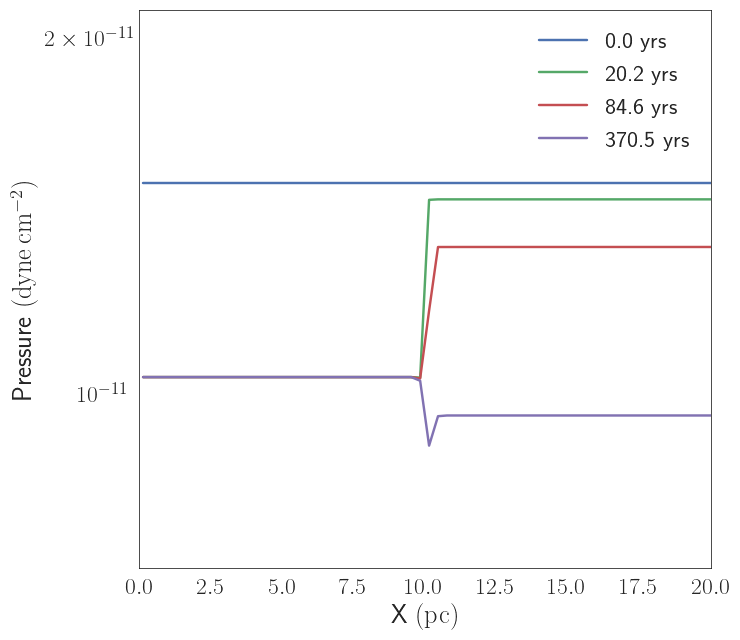
\includegraphics[width=1\linewidth]{DataImages/TabCoolingPRSprofile-micro}
%	\caption{Το προφίλ της πίεσης ενός νέφους με ενεργοποιημένο το Tabulated Cooling Module κατά μήκος της ευθείας $y=0$ με το χρόνο, σε τάξη εκατοντάδων ετών.}
%	\label{fig:tabcoolingprsprofile-micro}
%\end{adjustwidth}
%\end{figure}



	

	\subsubsection{Crossing Time}
%	Ο σκοπός μας είναι να εξετάζουμε βήμα - βήμα τη δυναμική των νεφών. Παρότι εντοπίσαμε το παραπάνω σφάλμα, το οποίο θα προσπαθήσουμε να λύσουμε με την εφαρμογή διαφορετικών modules ψύξης, θα εξετάσουμε ακόμα μια παράμετρο του γενικού μας προβλήματος.
%	
	 Από την εξίσωσης της ορμής:
	\begin{equation}
	\dv{\va V}{t}=-\frac{\grad P}{\rho}
	\end{equation}
	η διαφορά πίεσης που εμφανίζεται λόγο διαφορετικού ρυθμού (και κυρίως τερματισμού της) ψύξης των δύο αερίων δημιουργεί μια δύναμη ακτινικά προς τα έξω η οποία διαστέλλει το νέφους. Ουσιαστικά η διαστολή αυτή είναι η μετάδοση δύο κυμάτων. Ενός κύματος συμπύκνωσης προς το εξωτερικό το οποίο συνοδεύεται από ένα κύμα αραίωσης στο εσωτερικό. Δηλαδή εν τέλει έχουμε μια φαινομενική "κατάρρευση" του νέφους, αφού η φαινομενική ακτίνα του (δηλαδή η ακτίνα εκείνη που διατηρεί την αρχική πυκνότητα) μικραίνει.
	 
	Η ταχύτητα διάδοσης αυτής της "κατάρρευσης" δηλαδή η ταχύτητα διάδοσης των δύο κυμάτων είναι η ταχύτητα του ήχου στο εκάστοτε μέσο. Η τοπική ταχύτητα του ήχου είναι:
	\begin{equation}
	c_s=\sqrt{\gamma \frac{P}{\rho}}
	\end{equation}
	όπου $\gamma = 5/3$
	
	
	Από τις αρχικές συνθήκες (παράγραφος~\ref{par:InitialConditions}) οι τοπικές ταχύτητες του ήχου για το εσωτερικό και το εξωτερικό είναι:
	\begin{align}
	c_s &=\SI{1.2}{km.s^{-1}} \qq{(MC)} \\
	c_s &=\SI{38.7}{km.s^{-1}} \qq{(ISM)}
	\end{align}
	
	Καθώς η πίεση πέφτει, η ταχύτητα του ήχου στο νέφος μειώνεται κατά ένα παράγοντα $\sim 0.75^{1/2}=0.8$ δηλαδή περίπου $1\si{.km.s^{-1}}$.
	
%	\begin{marginfigure}
%		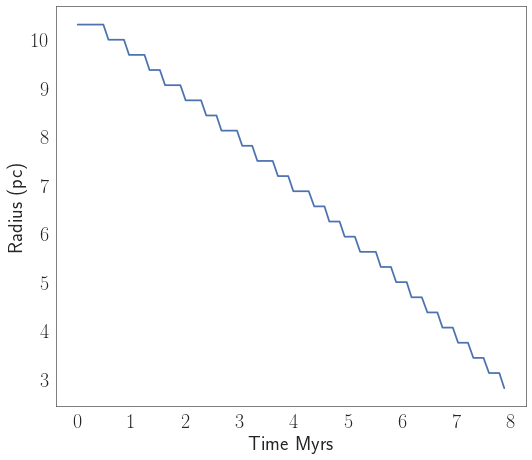
\includegraphics[width=1\linewidth]{DataImages/TabCoolingRadius}
%		\caption{Εκτίμηση της ακτίνας του νέφους συναρτήσει του χρόνου. Υπολογίστηκε με βάση τη παράγωγο του προφίλ της πυκνότητας κατά μήκος της ευθείας $y=0$}
%		\label{fig:tabcoolingradius}
%	\end{marginfigure}
%	
	Άρα τώρα μπορούμε να εκτιμήσουμε τη χρονική κλίμακα της "κατάρρευσης" με βάση την ακτίνα του νέφους:
	\begin{equation}
	\tau_R=\frac{R}{c_s} \simeq \SI{7.5}{\mega yrs}
	\end{equation}
	το οποίο φαίνεται να συμφωνεί με τη παρατήρηση, βλέπε σχήμα~\ref{fig:tabcoolingradius}.
	
	\subsubsection{Πρώτα Συμπεράσματα}
	Με τη χρήση του Tabulated Cooling Module του PLUTO δείξαμε ότι η προσπάθεια προσομοίωσης της δυναμική ενός σχετικά κρύου αερίου είναι εσφαλμένη καθώς οδηγεί σε μια κατώτατη θερμοκρασία η οποία προκύπτει από τα όρια του πίνακα θερμοκρασιών.
	
	Παρότι θα μπορούσαμε να επεκτείνουμε μέσω τεχνικών παρεμβολής τον πίνακα  $\Lambda (T)$ κρίναμε ότι κάτι τέτοιο απλά θα προσφέρει μια νέα χαμηλότερη θερμοκρασία και άρα μια επανάληψη των ίδιων περίπου αποτελεσμάτων με μια σχετική χρονική καθυστέρηση. 
	
	Άρα χρειαζόμαστε μια νέα προσέγγιση του όρου ψύξης στις χαμηλές θερμοκρασίες ώστε να αποκομίσουμε μια ρεαλιστικότερη απεικόνιση της εξέλιξης ενός κρύου αερίου μέσα στο διαγαλαξιακό μέσο.  
	
	Με βάση ένα εσφαλμένο μοντέλο έχουμε ενδείξεις για το πόσο σημαντικό ρόλο παίζει, σε νέφη τεραστίων διαστάσεων η ψύξη στις πολύ μικρές θερμοκρασίες. 
	
	\subsection{SNEq Cooling}
	Με βάση τα παραπάνω θα εξετάσουμε το δεύτερο module ψύξης μέσω ακτινοβολίας οπτικά αραιού μέσου του PLUTO, το οποίο ονομάζεται \textbf{Simplified Non-Equilibrium Cooling (SNEq)}. 
	
	Για να χρησιμοποιήσουμε το SNEq θα πρέπει να ορίσουμε σαν μια ακόμη μεταβλητή την
	αναλογία ουδετέρου Υδρογόνου σε σχέση με το Πλάσμα.
	Σε κάθε βήμα της προσομοίωσης ο κώδικας ολοκληρώνει μαζί με τις υδροδυναμικές εξισώσεις και την χρονική μεταβολή του $x_{H_I}$ μέσω της εξίσωσης:
	\begin{equation}
	\pdv{x_{\ce{HI}}}{t}=n_e \left( -(c_r+c_i)f_n+c_r\right) 
	\end{equation}
	μαζί με την εξίσωση της ενέργειας ή οποία γίνεται:
	\begin{equation}
	\pdv{t}(\rho e)=-\Lambda=-n_e n_H \left( \sum\limits_{k=1}^{16}j_k +w_{i/r} \right) 
	\end{equation}
	
	όπου η άθροιση στα $k$ υπολογίζει 16 διαφορετικές γραμμές εκπομπής 
	(Ly α, H α, HeI (584+623), CI (9850 + 9823), CII (156μ), CII (2325Å), NI (5200 Å),
	NII (6584 + 6548 Å), OI (63μ), OI (6300 + 6363 Å), OII (3727), MgII (2800), SiII (35μ), SII (6717 + 6727),FeII (25μ), FeII (1.6μ))
	\todo{Render line emmisions}
	
	Ο συντελεστής $j_k$ έχει μονάδες $\si{erg/sec . cm^3}$ και υπολογίζεται από τη σχέση:
	\begin{equation}
	j_k=\frac{\hbar^2 \sqrt{2\pi}}{\sqrt{k_B m_e}m_e}f_k q_{12}\frac{h \nu _k}{1+n_e (q_{21}/A_{21})}
	\end{equation}
	με $k$ τον δείκτη της εκάστοτε μετάπτωσης και $f_k=n_k/n_H$ το ποσοστό του εκάστοτε στοιχείου.
	\begin{align}
	q_{12}=\frac{\num{8.6e-6}}{\sqrt{T}}\frac{\Omega _{12}}{g_1}e^{-\frac{h\nu _k}{k_B T}} 
	&&
	q_{21}=\frac{\num{8.6e-6}}{\sqrt{T}}\frac{\Omega _{21}}{g_2}
	\end{align} 
	με $\Omega _{12} = \Omega _{21}$ η ισχύς της σύγκρουσης με τιμές οι οποίες είναι καταγεγραμμένες σε πίνακα.
	Το $w_{i/r}$ αντιπροσωπεύει τη θερμική ενέργεια που χάνεται από τον ιονισμό και την επανασύνδεση:
	\begin{equation}
	w_{i/r} = c_i\times \num{13.6}\times \num{1.6e-12} f_n +c_r \times \num{0.67}\times \num{1.6e-12} (1-f_n) \frac{T}{11590}
	\end{equation}
	όπου $c_r$ και $c_i$ είναι οι ρυθμοί ιονισμού και επανασύστασης του Υδρογόνου:
	\begin{align}
	c_r=\frac{\num{2.6e-11}}{\sqrt{T}} 
	&& 
	c_i=\frac{\num{1.08e-8}\sqrt{T}}{\num{13.6}^2} e^{-\frac{\num{157890}}{\sqrt{T}}}
	\end{align}
	
	
	\subsubsection{Προσομοίωση με SNEq Cooling}
	
			\begin{marginfigure}
				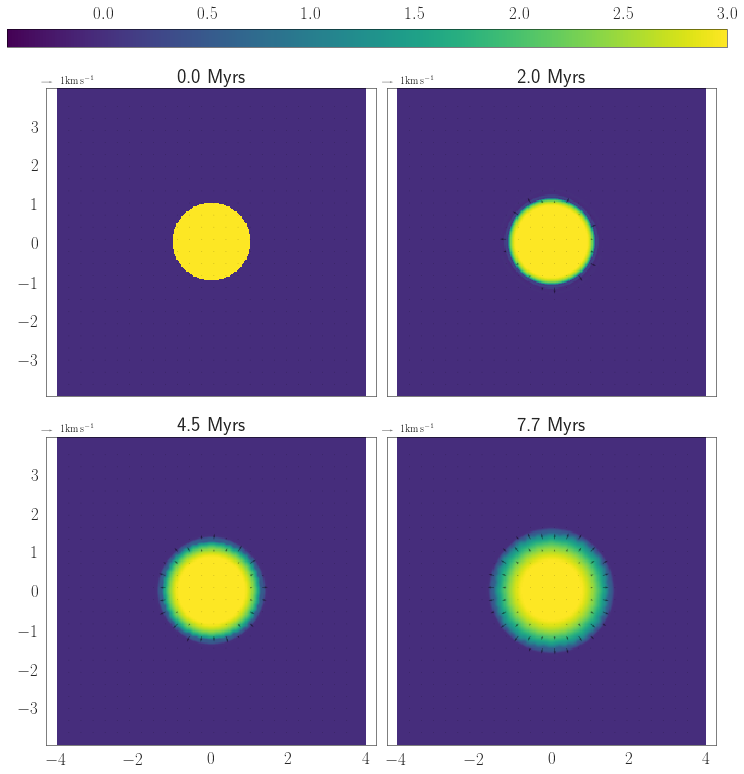
\includegraphics[width=1\linewidth]{DataImages/SNCoolingRHOquad}
				\caption{Ο χάρτης της πυκνότητας του νέφους για τη προσομοίωση του SNEq Cooling στο χρόνο (σε λογαριθμική κλίμακα).}
				\label{fig:sncoolingrhoquad}
			\end{marginfigure}
	
	Δεχόμενοι σαν βάση τη προηγούμενη προσπάθεια μας και τις ίδιες αρχικές συνθήκες για να χρησιμοποιήσουμε το SNEq Cooling Module θα πρέπει να ορίσουμε το ποσοστό ουδετέρου Υδρογόνου $x_{\ce{HI}}$.
	
	Για να ελέγξουμε την ευστάθεια των χημικών διεργασιών θεωρήσαμε σαν αρχική συνθήκη το ποσοστό του ουδετέρου υδρογόνου να είναι στο εσωτερικό του νέφους $x_{\ce{HI}}=0.1$ οπότε θα περιμέναμε λόγω της χαμηλής θερμοκρασίας και υψηλής πυκνότητας το ποσοστό αυτό να αυξηθεί. Στο εξωτερικό του νέφους, με το ίδιο σκεπτικό, χρησιμοποιούμε τη τιμή $x_{\ce{HI}}=0.9$ οπότε αντίστοιχα περιμένουμε λόγω της υψηλής θερμοκρασίας και της χαμηλής πυκνότητας σχεδόν ολόκληρο το υδρογόνου να είναι σε ατομική μορφή. 
	


	Όπως παρατηρούμε και από το σχήμα \ref{fig:sncoolingtmpcenterism} η συμπεριφορά είναι όντως η αναμενόμενη εκτός από το μεσοαστρικό χώρο ο οποίος κρυώνει σε πολύ μικρό χρονικό διάστημα αναγκάζοντας το ποσοστό ουδετέρου υδρογόνου να μειώνεται έως ότου η χαμηλή θερμοκρασία να το επαναφέρει στο 100\%. 
	
		\begin{marginfigure}
		\centering
		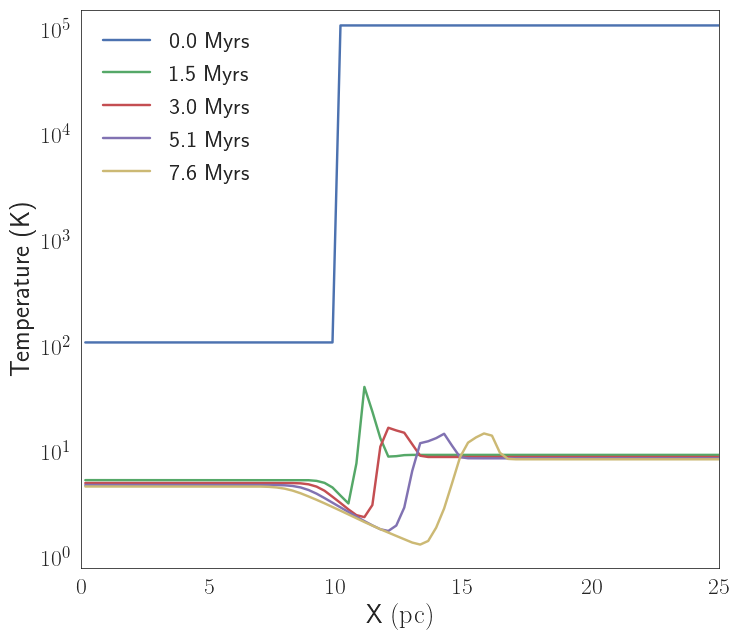
\includegraphics[width=1\linewidth]{DataImages/SNCoolingTMPprofile}
		\caption{}
		\label{fig:sncoolingtmpprofile}
	\end{marginfigure}
	
	\begin{marginfigure}
		\centering
		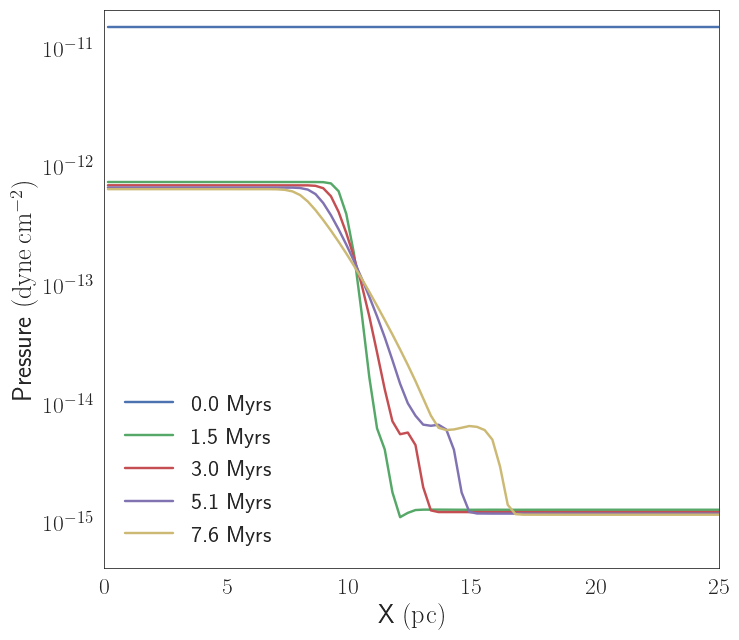
\includegraphics[width=1\linewidth]{DataImages/SNCoolingPRSprofile}
		\caption{}
		\label{fig:sncoolingprsprofile}
	\end{marginfigure}
	
\begin{figure}[h]
	\centering
	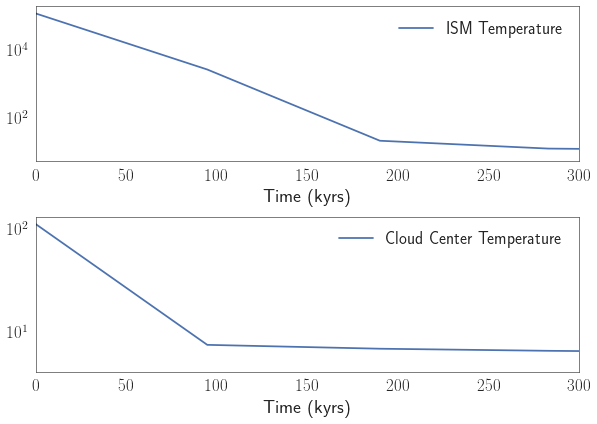
\includegraphics[width=1\linewidth]{DataImages/SNCoolingTMPcenterISM}
	\caption{Θερμοκρασία (αριστερή κλίμακα) και ποσοστό ουδετέρου υδρογόνου (διακεκομμένη καμπύλη, δεξιά κλίμακα) για το μεσοαστρικό αέριο (επάνω σχήμα) και εσωτερικό του νέφους (κάτω σχήμα)}
	\label{fig:sncoolingtmpcenterism} 
\end{figure}
	

Η θερμοκρασία του νέφους φτάνει σε τιμές κάτω των $\SI{10}{K}$ το οποίο έρχεται σε συμφωνία με τα  παρατηρησιακά δεδομένα από τα μοριακά νέφη. Όπως είδαμε και προηγουμένως η θερμοκρασία του μεσοαστρικού χώρου μειώνεται αρκετά γρήγορα κοντά στους \SI{10}{K}.
\todo[inline]{Γιατι ρε ΓΑΜΗΜΕΝΟ??}

Λόγω της σχεδόν ισοδύναμης ψύξης του νέφους με το μεσοαστρικό περιβάλλον η διαφορά πίεσης είναι μικρότερη όπως και η ταχύτητα του ήχου στο εσωτερικό του νέφους με αποτέλεσμα η φαινομενική κατάρρευση της κεντρικής περιοχής να είναι πολύ πιο αργή σε σχέση με το Tabulated Cooling. Στο σχήμα \ref{fig:tabsnsoundspeed} παρουσιάζουμε τις διαφορές στη ταχύτητα του ήχου μεταξύ του tabulated Cooling και του SNEq Cooling.

\begin{marginfigure}
	\centering
	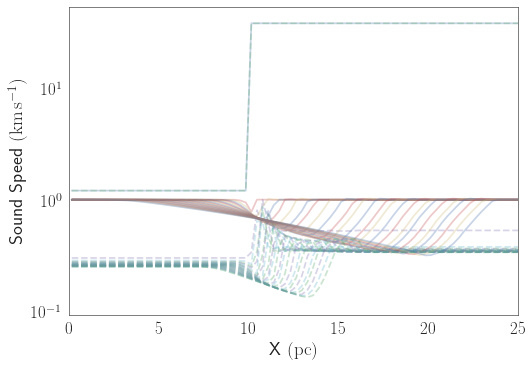
\includegraphics[width=1\linewidth]{DataImages/TabSNSoundSpeed}
	\caption{}
	\label{fig:tabsnsoundspeed}
\end{marginfigure}

Συμπερασματικά παρότι η ψύξη στο εσωτερικό του νέφους αποδίδει πιο ρεαλιστικά αποτελέσματα σε σχέση με τις παρατηρήσεις η \todo{αφου δεν εχουμε CO γιατί κρυώνει τόσο χαμηλα}


%	\begin{marginfigure}
%		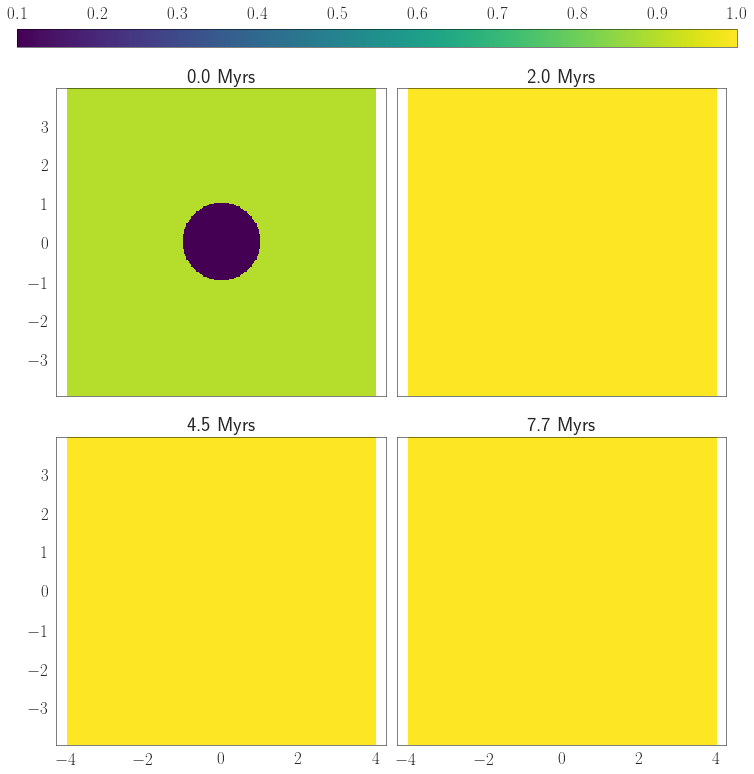
\includegraphics[width=1\linewidth]{DataImages/SNCoolingXHIquad}
%		\caption{Χρονική εξέλιξη του ποσοστού ουδετέρου Υδρογόνου}
%		\label{fig:sncoolingxhiquad}
%	\end{marginfigure}
%	

%\begin{figure}[h]
%	\begin{adjustwidth}{-0cm}{-5cm}	
%	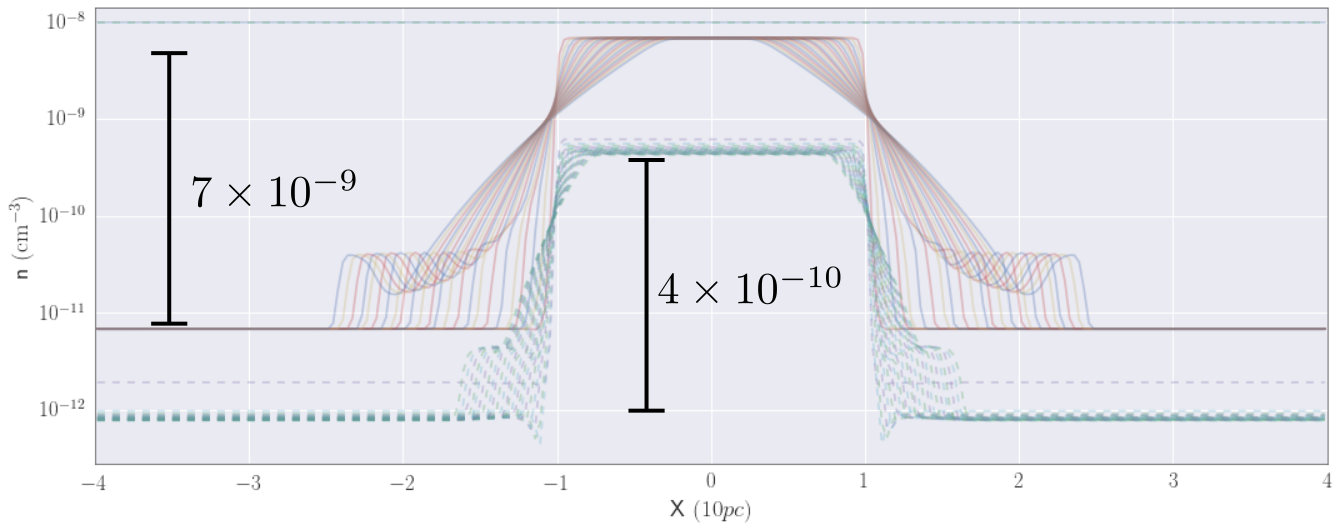
\includegraphics[width=1\linewidth]{DataImages/diffTabCoolSNCoolPRSprofile-edit}
%\caption{Το προφίλ της πίεσης του αερίου με ενεργοποιημένο το SNEq Cooling Module (διακεκομένη γραμμή) σε σύγκριση με αυτή του Tabulated Cooling κατά μήκος της ευθείας $y=0$ με το χρόνο.}
%\label{fig:difftabcoolsncoolprsprofile-edit}
%\end{adjustwidth}
%\end{figure}


\newpage
	\subsection{H2 Cooling}
%	Η ψύξη μέσω του SNEq είχε εμφανώς καλύτερα, δηλαδή πιο ρεαλιστικά αποτελέσματα αλλά διατηρεί ένα μεγάλο πρόβλημα που έχουμε για τις χαμηλές θερμοκρασίες. Οι μαγνητουδροδυναμικοί αριθμητικοί κώδικες αντιλαμβάνονται το ρευστό σαν ιονισμένο πλάσμα. Παρότι σε μεγάλες θερμοκρασίες η προσέγγιση αυτή είναι καλή σε χαμηλές θερμοκρασίες εμφανίζονται ουδέτερα άτομα και μόρια.
	
	Παρότι σε υψηλές θερμοκρασίες η προσέγγιση του αερίου σαν ιονισμένο πλάσμα είναι ικανοποιητική
	σε χαμηλές θερμοκρασίες όπου κυριαρχούν οι μοριακές εκπομπές είναι ανεπαρκής έως και λανθασμένη. Οι περισσότεροι μαγνητοϋδροδυναμικοί αριθμητικοί κώδικες όπως και ο PLUTO επιλύουν τις εξισώσεις μέ τη προσέγγιση του ενός ρευστού το οποίο σημαίνει ότι δυναμικά δεν μπορούμε να αποφύγουμε το μη υπολογισμό φαινομένων της αλληλεπίδρασης των πολλαπλών στοιχείων, μορίων και σκόνης (ειδικότερα αν βάλουμε στο παιχνίδι και μαγνητικά πεδία). 
	
	Tα Cooling modules SNEq και H2Cool δραστηριοποιούνται παράλληλα με την ολοκλήρωση των κινητικών εξισώσεων υπολογίζοντας την εξέλιξη της χημικής σύστασης του αερίου μέσω χημικών δικτύων και με βάση τη πυκνότητα και τη θερμοκρασία.  
	
%	Το SNEq module μέσω του χειρισμού του ποσοστού $x_{H_I}$ έκανε ένα βήμα προς αυτή τη κατεύθυνση αλλά για ένα μοριακό νέφος με μεγάλες ποσότητες σε \ce{H_2}, πληθώρα άλλων μορίων (\ce{He}, \ce{CO} κλπ) μαζί με σκόνη προφανώς η προσέγγιση αυτή δεν είναι αρκετή.
%	
%	Έτσι δοκιμάσαμε και το επόμενο Cooling Module που διαθέτει ο PLUTO το οποίο ονομάζεται \textbf{Molecular Hydrogen Non-Equilibrium Cooling (H2 COOL)}.
	
	Το H2COOL εισάγει με τη σειρά του 2 ακόμα μεταβλητές. Έτσι, εκτός του ποσοστού ουδετέρου υδρογόνου, έχουμε το ποσοστό ιονισμένου υδρογόνου $x_{H_{II}}$ και το ποσοστό μοριακού Υδρογόνου $x_{H_2}$.
	\begin{align}
	x_{H_I} =\frac{n_{H_I}}{n_H} && x_{H_I} =\frac{n_{H_{II}}}{n_H} && x_{H_2} =\frac{n_{H_2}}{n_H} 
	\end{align}
	όπου η συνολική αριθμητική πυκνότητα του Υδρογόνου $n_H=n_{H_I}+n_{H_{II}}+2n_{H_2}$.
	
	Η χημική εξέλιξη του μοριακού, ατομικού και ιονισμένου υδρογόνου ακολουθεί τις αντιδράσεις:
	\begin{align}
	&\ce{H + e^- -> H^+ + 2e^-} && k_1 = \num{5.84e-11} \sqrt{T} e^{\num{-157809}/T} \\
	&\ce{H^+ + e^- -> H + h\nu} && k_2 = \num{2.6e-11} \sqrt{T}\\
	&\ce{H_2 + e^- -> 2H + e^-} && k_3 = \num{4.4e-10}T^{0.35} e^{\num{-102000}/T}\\
	&\ce{H_2 + H -> 3H} && k_4=\num{1.067e-10}T_{eV}^{2.012} e^{\frac{\num{-4.463}}{T_{eV}}(1+\num{0.2472}T_{eV})^{3.512}}\\
	&\ce{H_2 + H_2 -> H_2 + 2H} && k_5=\num{1.0e-8}e^{-\num{84100}/T} \\
	&\ce{H + H ->[dust] H_2} && k_6=\num{3.0e-17}\sqrt{T_2} (1+0.4\sqrt{T_2}+0.2 T_2 +0.08 (T_2)^2)
	\end{align}
	όπου $T$ η θερμοκρασία σε Κέλβιν, $T_{eV}$ η θερμοκρασία σε ηλεκτρονιοβόλτ, $T_2=\frac{T}{100}$ και $k_i$ ο ρυθμός εξέλιξης της κάθε αντίδρασης σε $\si{cm^3 s^{-1}}$.
	
	Η εξέλιξη των αριθμητικών πυκνοτήτων υπολογίζεται από την εξίσωση:
	\begin{equation}
	S_i=\dv{n_i}{t}=\sum\limits_{j,k}k_{j,k}n_j n_k - n_i \sum_{j}k_{i,j}n_j
	\end{equation}
	\todo{Δεν είμαι σίγουρος οτι είναι ακρβωςο όρος $S_i$ }
	όπου $k_{j,k}$ είναι ο ρυθμός παραγωγής του $i$ στοιχείου από τα υπόλοιπα στοιχεία $j$ και $k$, και $k_{i,j}$ ο ρυθμός καταστροφής του $i$ στοιχείου από όλα τα $j$ στοιχεία.
	
	Ο κώδικας ολοκληρώνει τα ποσοστά των 3 ειδών υδρογόνου μέσω της επίλυσης της παραπάνω εξίσωσης μαζί με την εξίσωση μεταφοράς:
	\begin{equation}
	\pdv{X_i}{t}=-\va{u}\cdot \grad{X_i}+S_i
	\end{equation}
	όπου ο όρος μεταφοράς $-\va{u}\cdot \grad{X_i}$ ολοκληρώνεται μαζί με τις υδροδυναμικές εξισώσεις μάζας, ορμής (hydro step) ενώ ο όρος $S_i$ ολοκληρώνεται κατά το βήμα της ψύξης (cooling step).
	
	Οι ενεργειακές απώλειες λόγω ψύξης τελικά υπολογίζονται, εκτός από τις παραπάνω αντιδράσεις, από τις απώλειες ιονισμού λόγω κρούσης $\Lambda _{\mathtt{CI}}$ και επανασύνδεσης λόγω ακτινοβολίας $\Lambda _{\mathtt{RR}}$, απώλειες λόγω περιστροφής και ταλάντωσης (rotational-vibrational cooling) $\Lambda _{\mathtt{rotvib}}$ και διάσπασης (dissosiation) $\Lambda _{\mathtt{diss}}$ των μορίων \ce{H_2}, και της διαδικασίας αλληλεπίδρασης σκόνης-αερίου (gas-grain process) $\Lambda _{\mathtt{grain}}$.
	\begin{equation}
	\Lambda = \Lambda _{\mathtt{CI}} + \Lambda _{\mathtt{RR}} +\Lambda _{\mathtt{rotvib}} + \Lambda _{\mathtt{diss}} + \Lambda _{\mathtt{grain}}
	\end{equation}
	
	\todo[inline]{Depending on the requirement, the user can add more components to the cooling function, for e.g., cooling due to fixed fractions of standard molecules like CO, OH, H 2 O etc or contributions from collisional excitation of lines as indicated in the SNEq module.}
%
%	\begin{marginfigure}
%	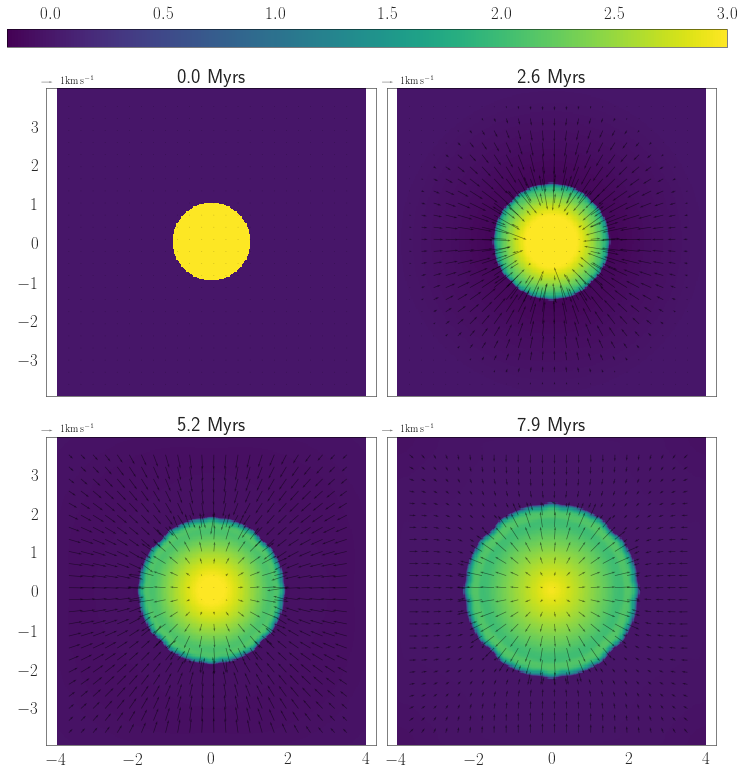
\includegraphics[width=1.\linewidth]{DataImages/H2CoolingRHOquad}
%	\caption{Η πυκνότητα του αερίου σε διάφορες χρονικές στιγμές}
%	\label{fig:h2coolingrhoquad}
%\end{marginfigure}	

	\subsubsection{Προσομοίωση με H2COOL}
		\marginpar{
		\begin{table}[H]
			\caption{Αρχικές συνθήκες για τα ποσοστά των διαφορετικών μορφών Υδρογόνου}
			\label{tab:h2sc}
			\begin{tabular}{|l|  c |  c| c|}
				\toprule
				Περιοχή & $x_{\ce{H_Ι}}$ & $x_{\ce{H_{ΙΙ}}}$ & $x_{\ce{H_2}}$ \\ 
				\midrule
				Μοριακό Nέφος & $0.1$ & $0$ & $0.9$ \\
				Μεσογαλαξιακό μέσο  & $0.9$ & $0.1$ & $0$ \\
				\bottomrule
			\end{tabular}
		\end{table}
	}

	Ακολουθώντας την ίδια πορεία με προηγουμένως ορίζουμε στις αρχικές συνθήκες τα ποσοστά μοριακού, ουδετέρου και ιονισμένου υδρογόνου όπως φαίνονται στο πίνακα~\ref{tab:h2sc}.
	
	\begin{marginfigure}
		\centering
		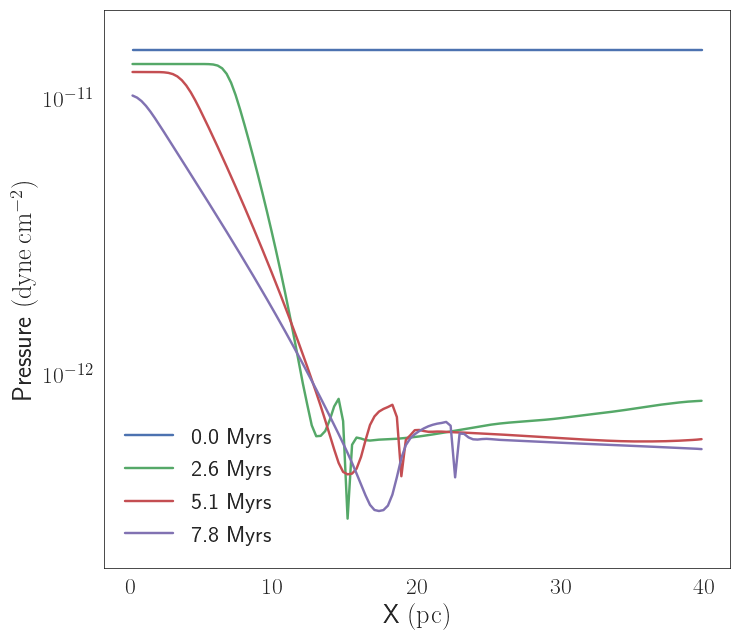
\includegraphics[width=1\linewidth]{DataImages/H2CoolingPRSprofile}
		\caption{}
		\label{fig:h2coolingprsprofile}
	\end{marginfigure}
	
	\begin{marginfigure}
		\centering
		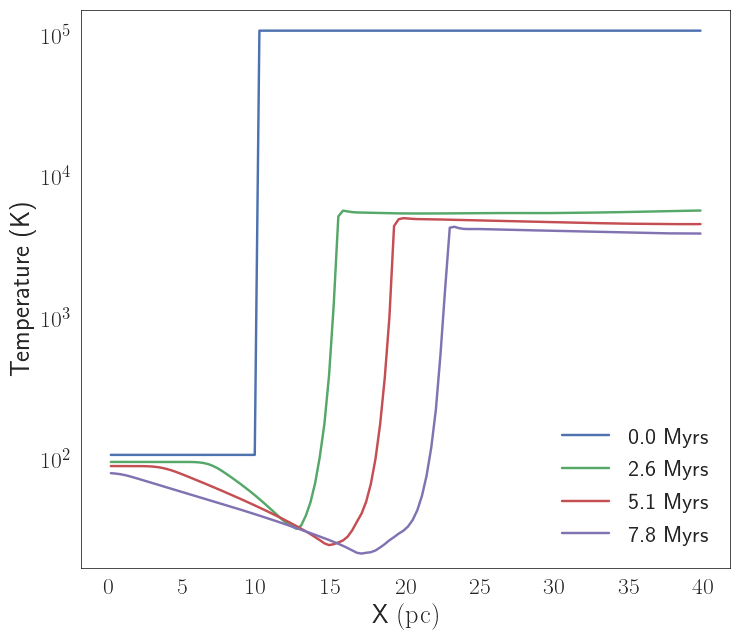
\includegraphics[width=1\linewidth]{DataImages/H2CoolingTMPprofile}
		\caption{}
		\label{fig:h2coolingtmpprofile}
	\end{marginfigure}
	
	
\begin{figure}[h]
	\centering
	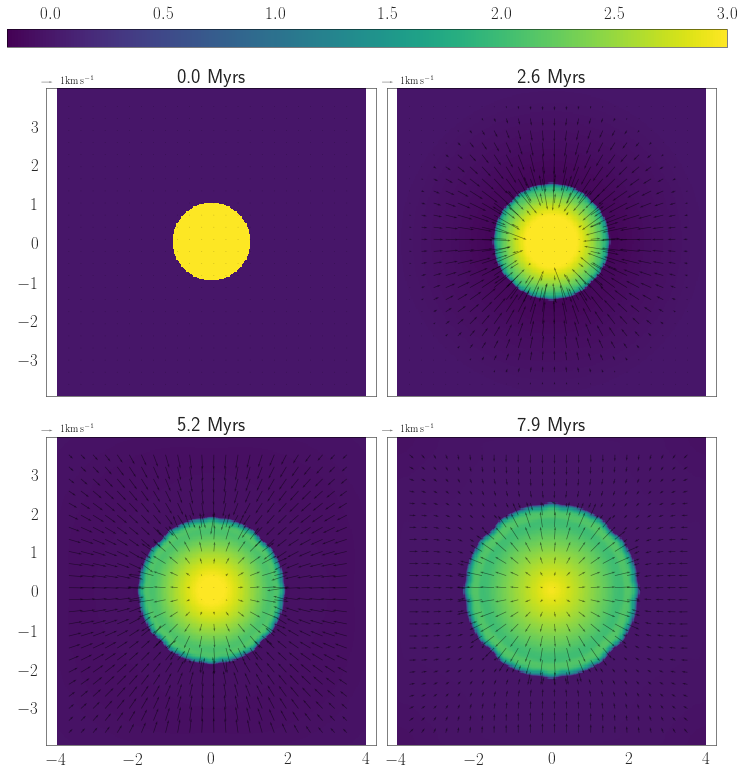
\includegraphics[width=1\linewidth]{DataImages/H2CoolingRHOquad}
	\caption{}
	\label{fig:h2coolingrhoquad}
\end{figure}


	Το πρώτο που παρατηρούμε είναι ότι το νέφος διαστέλλεται σε χρονική κλίμακα τάξης του crossing time. Ο λόγος είναι γιατί η διαφορά πιέσεων είναι πολύ μεγαλύτερη καθώς το κεντρικό τμήμα του νέφους διατηρεί τη πίεση στα ίδια επίπεδα με την αρχική πίεση $10^{-8}$. Για να αλλάξει η πυκνότητα στο εσωτερικό του νέφους χρειάζεται ένας αρκετά μεγάλος χρόνος, άρα η σχετική στασιμότητα της πίεσης σημαίνει και στασιμότητα της θερμοκρασίας. Όντως όπως βλέπουμε και στο σχήμα~\ref{fig:h2coolingtmpprofile} η θερμοκρασία του νέφους διατηρείται κοντά 
στην αρχική τιμή των $\SI{100}{K}$.

	Ενώ για το διαγαλαξιακό μέσο ο ρυθμός ψύξης φαίνεται να επιβραδύνεται αρκετά κοντά στους $\SI{3e3}{K}$ καθώς ολόκληρο το υδρογόνο μετατρέπεται σε ουδέτερο (σχήμα \ref{fig:h2coolingtmpcenterism}).

\begin{figure}
	\centering
	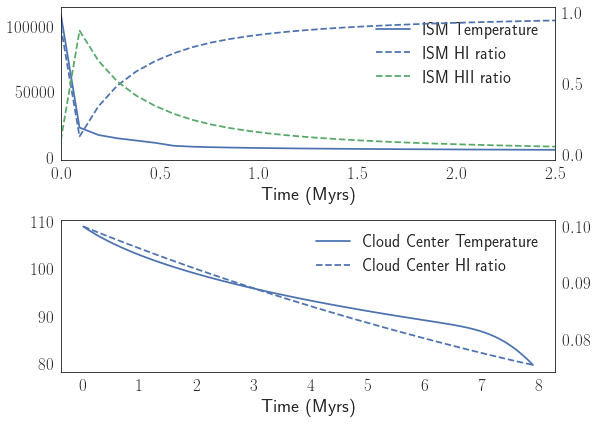
\includegraphics[width=1\linewidth]{DataImages/H2CoolingTMPcenterISM}
	\caption{}
	\label{fig:h2coolingtmpcenterism}
\end{figure}


	Οι παρατηρήσεις των μοριακών νεφών μας δίνουν θερμοκρασίες της τάξεως των $\SI{30}{K}$. Η ασυμφωνία με την προσομοίωση εξηγείται καθώς το module H2COOL απευθύνεται αυστηρά στις μεταβάσεις και μεταβολές του Υδρογόνου. Οι ενεργειακές μεταβάσεις του υδρογόνου είναι σημαντικές για θερμοκρασίες περίπου πάνω από $\SI{100}{K}$. Για χαμηλότερες θερμοκρασίες κυρίαρχο ρόλο παίζουν τα \ce{CO}, \ce{OH}, \ce{H2O} και \ce{He}
	
Αν χρησιμοποιούσαμε χαμηλότερη θερμοκρασία (για παράδειγμα τους \SI{30}{K}) τότε το αέριο θα διατηρούταν σε αυτή τη θερμοκρασία. Επειδή όμως θέλαμε να μελετήσουμε τη ψύξη στο νέφος αποφύγαμε να "επιβάλλουμε" τη δική μας αποδεκτή θερμοκρασία.

\begin{figure}[h]
	\centering
	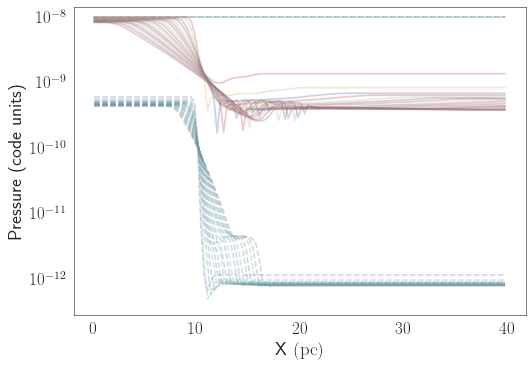
\includegraphics[width=1\linewidth]{DataImages/diffH2CoolSNCoolPRSprofile.png}
	\caption{}
	\label{fig:diffh2coolsncoolprsprofile}
\end{figure}




	\newpage
	\section{Βαρύτητα}
	Είναι προφανές ότι έναν από τους ισχυρότερους ρόλους στην αστροφυσική (αν όχι το μεγαλύτερο) τον παίζει η βαρύτητα. 
	
	\subsection{Self Gravity}
	\label{par:SolidSphereSelfGravit}
	Επειδή ο PLUTO δεν μπορεί να χειριστεί την ιδιοβαρύτητα θα προσπαθήσουμε να τη προσεγγίσουμε τοποθετώντας ένα βαρυτικό δυναμικό ομογενούς σφαίρας στο εσωτερικό του νέφους και ένα δυναμικό σημειακής μάζας στο εξωτερικό του νέφους. Δηλαδή:
	\begin{equation}
		\vec{g}(x,y) = 
		\begin{cases}
			\frac{GM}{R^3}(x \hat{x}+ y \hat{y}) &\texttt{if } r<R \\
			\frac{GM}{r^3}(x \hat{x}+ y \hat{y}) &\texttt{if } r>R
		\end{cases}
	\end{equation}
	
	όπου $r=\sqrt{x^2+y^2}$
	
	\subsubsection{Βαρυτική Σταθερά}
	Για να χρησιμοποιήσουμε τη δύναμη της βαρύτητας θα πρέπει να υπολογίσουμε τη σταθερά $G$ σε μονάδες κώδικα, όπως βλέπουμε και από το πίνακα~\ref{tab:cd}. Άρα 
	\begin{equation}
		G=G_\texttt{cgs} \si{cm^3.g^{-1}.s^{-2}} = G_\texttt{cgs} \frac{\SI{1.67e-24}{g.cm^{-3}}}{\rho_0}\frac{10^{18}\si{s^2}}{t^2_0}
	\end{equation}
	Αντικαθιστώντας $G_\texttt{cgs}=\SI{6.674e-8}{}$ βρίσκουμε
	\begin{equation}
		\boxed{G=\SI{1.114e-13}{G_0}}
	\end{equation}
	όπου $G_0=(\rho_0 t_0)^{-1}$ η σταθερά της βαρύτητας σε μονάδες κώδικα.
	
%	\begin{marginfigure}
%		\includegraphics[width=1.0\linewidth]{astro/Diplomatiki/logDensityG}
%		\caption{Density Simulation (Logarithmic Scale) over four different times in one $t_\texttt{ff}$.}
%		\label{fig:logdensityg}
%	\end{marginfigure}
	
	\subsubsection{Χρόνος Ελεύθερης Πτώσης}
	Ο χρόνος ελεύθερης πτώσης (free-fall time) είναι η χρονική κλίμακα που χρειάζεται ένα σώμα να καταρρεύσει κάτω από το ίδιο το βάρος του, αν δεν υπεισέρχονται άλλες δυνάμεις που να αντισταθμίσουν ή να επιταχύνουν τη διαδικασία. Έτσι παίζει ένα πολύ σημαντικό ρόλο στις χρονικές κλίμακες πολλών αστροφυσικών διεργασιών.
	
	Στη περίπτωση του δικού μας νέφους ο χρόνος ελεύθερης πτώσης υπολογίζεται:
	\begin{equation}
		t_\texttt{ff}=\sqrt{\frac{3\pi}{32G\rho}} = \SI{51404}{t_0} = \SI{1.6}{Myrs}
	\end{equation}
	
	\subsection{Σφαιρικό νέφος μέσα σε βαρυτικό δυναμικό χωρίς Ψύξη}
	
	Για να εξετάσουμε την επίδραση της βαρύτητας αρχικά θα εκτελέσουμε την προσομοίωση που έχουμε κάνει και προηγουμένως, αρχικά σε ένα νέφος που δεν εμπεριέχει διαδικασία ψύξης.
	
\begin{figure}[h]
	\centering
	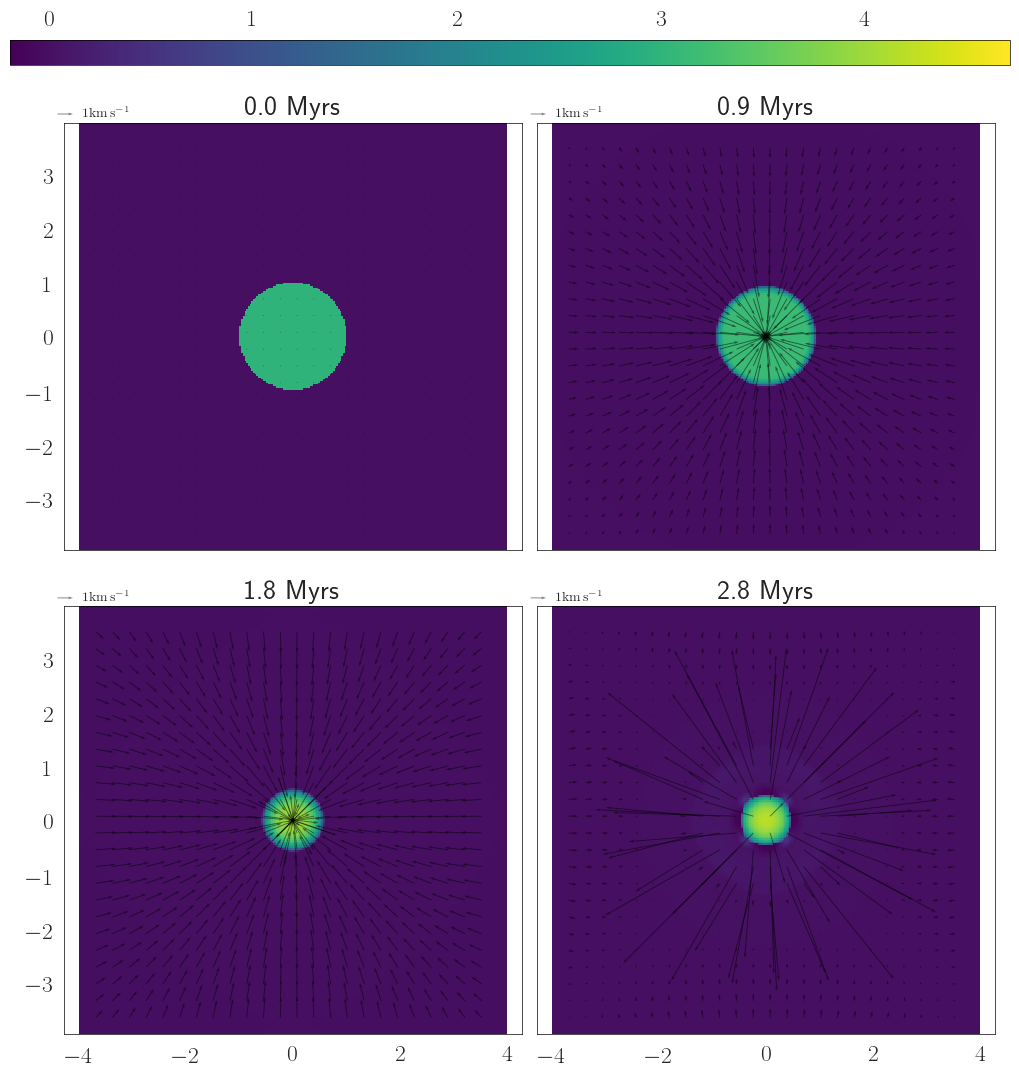
\includegraphics[width=1\linewidth]{DataImages/NoCoolGRquad}
	\caption{}
	\label{fig:nocoolgrquad}
\end{figure}

\begin{marginfigure}
	\centering
	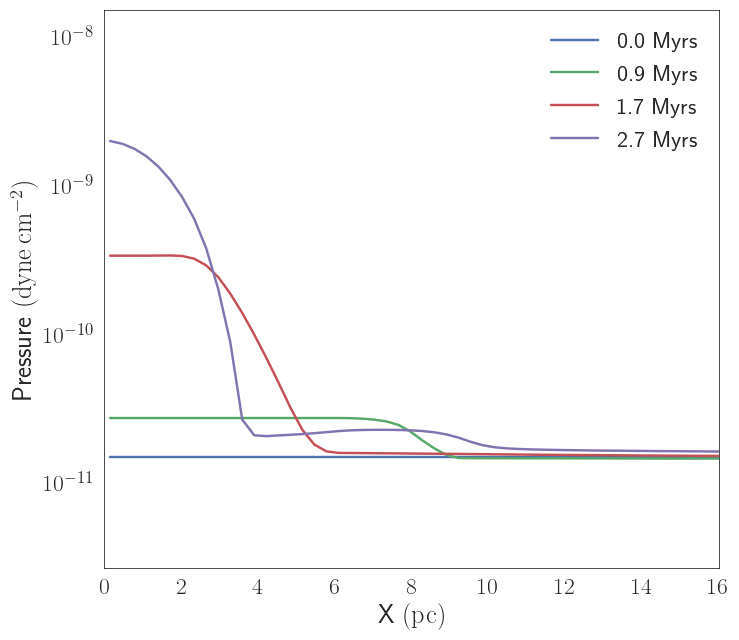
\includegraphics[width=1\linewidth]{DataImages/NoCoolGPRSprofile.png}
	\caption{}
	\label{fig:nocoolgprsprofile}
\end{marginfigure}

Το αποτέλεσμα όπως φαίνεται από το σχήμα~\ref{fig:nocoolgrhoprofile} δείχνουν ένα χρόνο κατάρρευσης κοντά στα $\SI{2}{Myrs}$ καθώς στη συνέχεια το νέφος αναπηδά λόγω της θερμικής πίεσης (σχήμα~\ref{fig:nocoolgprsprofile}) και επιταχύνεται προς τα έξω.
Το αποτέλεσμα είναι πολύ κοντά στην τιμή του χρόνου ελεύθερης πτώσης καθώς η πίεση δεν ήταν αρκετή για να επιβραδύνει νωρίτερα την κατάρρευση και επίσης η ακρίβεια των προσομοιώσεων δεν είναι αρκετή για να διαχειρίστει απόλυτα σωστά το φαίνομενο της βαρυτικής κατάρρευσης. Ένα pixel αντιστοιχεί σε $\SI{0.3125}{parsec}\simeq \SI{1}{ly}$ μέγεθος πολύ μεγαλύτερο από ένα πρωτοαστέρα.

\subsection{Σφαιρικό νέφος με Radiation Cooling με ιδιοβαρύτητα}

Στη συνέχεια θα επαναλάβουμε τη προσομοίωση της βαρυτικής κατάρρευσης μαζί με τη ψύξη του αερίου

 χρησιμοποιήσουμε 
Θεωρώντας μέχρι στιγμής το πιο ρεαλιστικό προσομοιωτή ψύξης αυτό του H2COOL, θα δοκιμάσουμε να επαναλάβουμε τη προσομοίωση μέσα σε δυναμικό ιδιοβαρύτητας έτσι όπως ορίστηκε στη παράγραφο~\ref{par:SolidSphereSelfGravit}. 
%
%	\subsubsection{Jeans Radius} 
%	\todo[inline]{λάθος ο υπολογισμός}
%	From the momentum equation we can estimate a critical Radius of a solid cloud by solving the equation:
%	\begin{equation}
%		\frac{\grad P}{\rho}=\frac{GM}{R^3}r 
%	\end{equation}
%	Where we can make an order of magnitude estimation:
%	\begin{equation}
%		\frac{P}{r^* \rho}=\frac{GM}{R^3}r^* \rightarrow \boxed{r^*=\left( \frac{PR^3}{G\rho ^2}\right) ^{1/5}}
%	\end{equation}
%	
%	For our cloud this calculation gives a critical radius of $\SI{4.6}{pc}$
%	
	
	\subsubsection{Σφαίρα Bonnor-Ebert}
	Η σφαίρα Bonnor-Ebert είναι η θεωρητική κατασκευή μιας ισόθερμης σφαίρας όπου η βαρύτητα εξισορροπείται από την εσωτερική πίεση. Δηλαδή ισχύουν οι εξισώσεις:
	\begin{align}
	\frac{Gm}{r^2} &+\frac{1}{\rho}\frac{dP}{dr}=0 \text{ Εξίσωση Κίνησης}\\
	\frac{dm}{dr} &= 4 \pi r^2 \rho \text{ Εξίσωση διατήρησης της Μάζας}\\
	P &= c_s ^2 \rho \text{ Καταστατική Εξίσωση}
	\end{align}
	
	Συνδυάζοντας και τις τρείς έχουμε:
	\begin{equation}
	\frac{1}{r^2}\frac{d}{dr} \left( r^2 c_s ^2 \frac{d \ln \rho}{dr}\right)  = -4 \pi G \rho
	\end{equation}
	
	Η λύση της οποίας μας δίνει τη πυκνότητα συναρτήση της ακτίνας μέσα στο μοριακό πυρήνα:
	\begin{equation}
	\label{eq:B-E_density}
	\rho (r) =\frac{c_s ^2}{2 \pi G} \frac{1}{r^2}
	\end{equation}
	
	
\section{Αλληλεπίδραση νέφους με Jet}
Το επόμενο βήμα 

Εφόσον έχουμε μια 


\end{document}